\edef\result#1{%
\ifstrequal{#1}{fft-mlc-cycles}{2.68}{}%
\ifstrequal{#1}{fft-mlc-error}{1\%}{}%
\ifstrequal{#1}{fft-mlc-speedup}{1.13$\times$}{}%
\ifstrequal{#1}{fft-mlc-stripe-cycles}{2.44}{}%
\ifstrequal{#1}{fft-mlc-stripe-error}{4\%}{}%
\ifstrequal{#1}{fft-mlc-stripe-speedup}{1.24$\times$}{}%
\ifstrequal{#1}{image-mlc-cycles}{1.41}{}%
\ifstrequal{#1}{image-mlc-error}{1\%}{}%
\ifstrequal{#1}{image-mlc-flash-cycles}{13.0}{}%
\ifstrequal{#1}{image-mlc-flash-error}{9\%}{}%
\ifstrequal{#1}{image-mlc-flash-speedup}{1.6$\times$}{}%
\ifstrequal{#1}{image-mlc-speedup}{2.14$\times$}{}%
\ifstrequal{#1}{image-mlc-stripe-cycles}{1.41}{}%
\ifstrequal{#1}{image-mlc-stripe-error}{1\%}{}%
\ifstrequal{#1}{image-mlc-stripe-speedup}{2.14$\times$}{}%
\ifstrequal{#1}{jmeint-mlc-cycles}{1.87}{}%
\ifstrequal{#1}{jmeint-mlc-error}{2\%}{}%
\ifstrequal{#1}{jmeint-mlc-speedup}{1.62$\times$}{}%
\ifstrequal{#1}{jmeint-mlc-stripe-cycles}{1.71}{}%
\ifstrequal{#1}{jmeint-mlc-stripe-error}{10\%}{}%
\ifstrequal{#1}{jmeint-mlc-stripe-speedup}{1.77$\times$}{}%
\ifstrequal{#1}{lu-mlc-cycles}{1.98}{}%
\ifstrequal{#1}{lu-mlc-error}{6\%}{}%
\ifstrequal{#1}{lu-mlc-speedup}{1.53$\times$}{}%
\ifstrequal{#1}{lu-mlc-stripe-cycles}{1.98}{}%
\ifstrequal{#1}{lu-mlc-stripe-error}{5\%}{}%
\ifstrequal{#1}{lu-mlc-stripe-speedup}{1.53$\times$}{}%
\ifstrequal{#1}{mc-mlc-cycles}{1.71}{}%
\ifstrequal{#1}{mc-mlc-error}{4\%}{}%
\ifstrequal{#1}{mc-mlc-speedup}{1.77$\times$}{}%
\ifstrequal{#1}{mc-mlc-stripe-cycles}{1.59}{}%
\ifstrequal{#1}{mc-mlc-stripe-error}{10\%}{}%
\ifstrequal{#1}{mc-mlc-stripe-speedup}{1.91$\times$}{}%
\ifstrequal{#1}{ml-mlc-cycles}{1.71}{}%
\ifstrequal{#1}{ml-mlc-error}{6\%}{}%
\ifstrequal{#1}{ml-mlc-flash-cycles}{19.7}{}%
\ifstrequal{#1}{ml-mlc-flash-error}{8\%}{}%
\ifstrequal{#1}{ml-mlc-flash-speedup}{1.05$\times$}{}%
\ifstrequal{#1}{ml-mlc-speedup}{1.77$\times$}{}%
\ifstrequal{#1}{ml-mlc-stripe-cycles}{1.41}{}%
\ifstrequal{#1}{ml-mlc-stripe-error}{0\%}{}%
\ifstrequal{#1}{ml-mlc-stripe-speedup}{2.14$\times$}{}%
\ifstrequal{#1}{mlc-flash-mean-cycles}{16.4}{}%
\ifstrequal{#1}{mlc-flash-mean-speedup}{1.26$\times$}{}%
\ifstrequal{#1}{mlc-mean-cycles}{1.91}{}%
\ifstrequal{#1}{mlc-mean-speedup}{1.59$\times$}{}%
\ifstrequal{#1}{mlc-stripe-mean-cycles}{1.79}{}%
\ifstrequal{#1}{mlc-stripe-mean-speedup}{1.7$\times$}{}%
\ifstrequal{#1}{nn-mlc-cycles}{1.87}{}%
\ifstrequal{#1}{nn-mlc-error}{1\%}{}%
\ifstrequal{#1}{nn-mlc-flash-cycles}{16.5}{}%
\ifstrequal{#1}{nn-mlc-flash-error}{10\%}{}%
\ifstrequal{#1}{nn-mlc-flash-speedup}{1.26$\times$}{}%
\ifstrequal{#1}{nn-mlc-speedup}{1.62$\times$}{}%
\ifstrequal{#1}{nn-mlc-stripe-cycles}{1.71}{}%
\ifstrequal{#1}{nn-mlc-stripe-error}{1\%}{}%
\ifstrequal{#1}{nn-mlc-stripe-speedup}{1.77$\times$}{}%
\ifstrequal{#1}{pa-mlc-cycles}{1.71}{}%
\ifstrequal{#1}{pa-mlc-error}{3\%}{}%
\ifstrequal{#1}{pa-mlc-flash-cycles}{16.5}{}%
\ifstrequal{#1}{pa-mlc-flash-error}{6\%}{}%
\ifstrequal{#1}{pa-mlc-flash-speedup}{1.26$\times$}{}%
\ifstrequal{#1}{pa-mlc-speedup}{1.77$\times$}{}%
\ifstrequal{#1}{pa-mlc-stripe-cycles}{1.59}{}%
\ifstrequal{#1}{pa-mlc-stripe-error}{5\%}{}%
\ifstrequal{#1}{pa-mlc-stripe-speedup}{1.91$\times$}{}%
\ifstrequal{#1}{raytracer-mlc-cycles}{1.59}{}%
\ifstrequal{#1}{raytracer-mlc-error}{7\%}{}%
\ifstrequal{#1}{raytracer-mlc-speedup}{1.91$\times$}{}%
\ifstrequal{#1}{raytracer-mlc-stripe-cycles}{1.59}{}%
\ifstrequal{#1}{raytracer-mlc-stripe-error}{6\%}{}%
\ifstrequal{#1}{raytracer-mlc-stripe-speedup}{1.91$\times$}{}%
\ifstrequal{#1}{recycle-fft-qos-ext}{5\%}{}%
\ifstrequal{#1}{recycle-fft-total-ext}{34\%}{}%
\ifstrequal{#1}{recycle-image-ext}{90\%}{}%
\ifstrequal{#1}{recycle-jmeint-qos-ext}{25\%}{}%
\ifstrequal{#1}{recycle-jmeint-total-ext}{34\%}{}%
\ifstrequal{#1}{recycle-lu-qos-ext}{11\%}{}%
\ifstrequal{#1}{recycle-lu-total-ext}{32\%}{}%
\ifstrequal{#1}{recycle-mc-qos-ext}{32\%}{}%
\ifstrequal{#1}{recycle-mc-total-ext}{34\%}{}%
\ifstrequal{#1}{recycle-mean-all-ext}{23\%}{}%
\ifstrequal{#1}{recycle-mean-nv-ext}{36\%}{}%
\ifstrequal{#1}{recycle-mean-qos-ext}{18\%}{}%
\ifstrequal{#1}{recycle-mean-total-ext}{34\%}{}%
\ifstrequal{#1}{recycle-ml-ext}{17\%}{}%
\ifstrequal{#1}{recycle-nn-ext}{17\%}{}%
\ifstrequal{#1}{recycle-pa-ext}{42\%}{}%
\ifstrequal{#1}{recycle-raytracer-qos-ext}{39\%}{}%
\ifstrequal{#1}{recycle-raytracer-total-ext}{39\%}{}%
\ifstrequal{#1}{recycle-smm-qos-ext}{20\%}{}%
\ifstrequal{#1}{recycle-smm-total-ext}{29\%}{}%
\ifstrequal{#1}{recycle-sor-qos-ext}{20\%}{}%
\ifstrequal{#1}{recycle-sor-total-ext}{32\%}{}%
\ifstrequal{#1}{recycle-zxing-qos-ext}{2\%}{}%
\ifstrequal{#1}{recycle-zxing-total-ext}{37\%}{}%
\ifstrequal{#1}{smm-mlc-cycles}{1.87}{}%
\ifstrequal{#1}{smm-mlc-error}{3\%}{}%
\ifstrequal{#1}{smm-mlc-speedup}{1.62$\times$}{}%
\ifstrequal{#1}{smm-mlc-stripe-cycles}{1.87}{}%
\ifstrequal{#1}{smm-mlc-stripe-error}{2\%}{}%
\ifstrequal{#1}{smm-mlc-stripe-speedup}{1.62$\times$}{}%
\ifstrequal{#1}{sor-mlc-cycles}{2.25}{}%
\ifstrequal{#1}{sor-mlc-error}{3\%}{}%
\ifstrequal{#1}{sor-mlc-speedup}{1.35$\times$}{}%
\ifstrequal{#1}{sor-mlc-stripe-cycles}{2.1}{}%
\ifstrequal{#1}{sor-mlc-stripe-error}{7\%}{}%
\ifstrequal{#1}{sor-mlc-stripe-speedup}{1.44$\times$}{}%
\ifstrequal{#1}{zxing-mlc-cycles}{2.25}{}%
\ifstrequal{#1}{zxing-mlc-error}{4\%}{}%
\ifstrequal{#1}{zxing-mlc-speedup}{1.35$\times$}{}%
\ifstrequal{#1}{zxing-mlc-stripe-cycles}{2.1}{}%
\ifstrequal{#1}{zxing-mlc-stripe-error}{9\%}{}%
\ifstrequal{#1}{zxing-mlc-stripe-speedup}{1.44$\times$}{}%
}


\section{Introduction}
\label{approxstorage:sec:intro}

Many common applications have intrinsic tolerance to inaccuracies in
computation. Techniques under the umbrella of {\em approximate
computing}~\cite{enerj,truffle,pcmos,green,stochasticproc,relax,perforation,flikker,ersa} exploit this tolerance
to trade off accuracy for performance or energy efficiency. Applications
in domains like computer vision, media processing, machine learning, and
sensor data analysis can see large efficiency gains in exchange for
small compromises on computational accuracy. This trade-off extends to
storage: error tolerance in both transient and persistent data is
present in a broad range of application domains, from server software to
mobile applications.

Meanwhile, the semiconductor industry is beginning to encounter limits to
further scaling of common memory technologies like DRAM and Flash. As a
result, new memory technologies and techniques are emerging. Multi-level cells,
which pack more than one bit of information in a single cell,
are already commonplace and phase-change memory (PCM) is imminent.
But both
PCM and Flash wear out over time as cells degrade and become unusable. Furthermore, multi-level cells
are slower to write due to the need for tightly
controlled iterative programming.

Memories traditionally address wear-out issues and implement multi-level cell
operation in ways that ensure perfect data integrity 100\% of the time. This
has significant costs in performance, energy, area, and complexity. These
costs are exacerbated as memories move to smaller device feature sizes along
with more process variation. By relaxing the requirement for perfectly precise
storage---and exploiting the inherent error tolerance of approximate
applications---failure-prone and multi-level memories can gain back
performance, energy, and capacity.

We propose techniques that exploit data accuracy trade-offs to
provide \emph{approximate storage}. In essence, we advocate exposing storage
errors up to the application with the goal of making data storage more
efficient. We make this safe by: (1) exploiting application-level inherent
tolerance to inaccuracies; and (2) providing an interface that lets the
application control which pieces of data can be subject to inaccuracies while offering error-free operation for the rest of the data.
We propose two basic techniques. The first
technique uses multi-level cells in a way that enables higher density or
better performance at the cost of occasional inaccurate data retrieval. The
second technique uses blocks with failed bits to store approximate data; to
mitigate the effect of failed bits on overall value precision, we prioritize
the correction of higher-order bits.

Approximate storage applies to both persistent storage (files or databases) as well as transient
data stored in main memory.
We explore the techniques in the context of PCM, which may be used for
persistent storage (replacing hard disks) or as main memory
(replacing DRAM)~\cite{pcm-dram-alt,durable-pcm-mm,qureshi-pcm-mm},
but the techniques generalize to other technologies such as Flash.
We simulate main-memory benchmarks and
persistent-storage datasets and find that our techniques improve write
latencies by \result{mlc-stripe-mean-speedup} or extend device lifetime by
\result{recycle-mean-all-ext} on
average while trading off less than 10\% of each application's output quality.

We begin by describing the programming models and hardware--software interfaces
we assume for main-memory and persistent approximate storage. Next,
Sections~\ref{approxstorage:sec:amlc} and~\ref{approxstorage:sec:recycling} describe our two
approximate-storage techniques in detail. Section~\ref{approxstorage:sec:eval} describes our
evaluation of the techniques using a variety of error-tolerant
benchmarks and Section~\ref{approxstorage:sec:results} gives the results for these
experiments. Finally, we enumerate related work on storage and approximate
computing and conclude.

\section{Interfaces for Approximate Storage}
\label{approxstorage:sec:idea}

% what we need: interface, mechanisms. interface needs as way to specific which bits matter more.
% who keeps track of what is approximate: SW knows. HW does not keep track of that. simplifies bookkeeping.

\emph{Approximate computing} lets programs
eschew traditional guarantees of perfect precision when they are
unnecessary. If a large portion of a program's work is
error-tolerant, the hardware can operate more
efficiently~\cite{flikker,truffle,pcmos,stochasticproc,relax}.
While previous work has considered reducing the energy spent on DRAM
and SRAM storage~\cite{flikker,enerj,truffle}, modern non-volatile
memory technologies also exhibit properties that make them candidates
for storing data approximately. By exploiting the synergy between
these properties and application-level error tolerance, we can alleviate
some of these technologies' limitations: limited device
lifetime, low density, and slow writes.

Approximate storage augments memory modules with software-visible
precision modes. When an application needs strict data fidelity,
it uses traditional \emph{precise} storage; the memory then
guarantees a low error rate when recovering the data. When the
application can tolerate occasional errors in some data, it uses
the memory's \emph{approximate} mode, in which data recovery errors
may occur with non-negligible probability.

This work examines the potential for approximate storage in
PCM and other solid-state, non-volatile memories.
These technologies have the potential to provide persistent mass storage
and to serve as main memory.
For either use case, the application must determine which data can
tolerate errors and which data needs ``perfect'' fidelity. As with
previous work that exposes approximation to software, we assume that
programmers need to make this decision---approximating data
indiscriminately can lead to broken systems~\cite{enerj,relax,green,truffle,npu}.

The next sections describe the approximation-aware programming
models for main memory and persistent mass storage along with
the hardware--software interface features common to both settings. 
In general,
each block (of some appropriate granularity) is logically in either
\emph{precise} or
\emph{approximate} state at any given time. Every read and write operation specifies
whether the access is approximate or precise.
These per-request precision flags allow the storage array to
avoid the overhead of storing per-block metadata. The
compiler and runtime are responsible for keeping track of which locations hold approximate
data. Additionally, the interface may also allow
software to convey the relative importance of bits within a block, enabling
more significant bits to be stored with higher accuracy.

Prior work on approximate computing has suggested that different applications
can tolerate different error rates~\cite{enerj,truffle} and our experimental
results (Section~\ref{approxstorage:sec:results}) corroborate this. However, rather than
providing interfaces to control precision levels at a fine grain, we apply a
uniform policy to all approximate data in the program.
Empirically, we find 
that this level of control is sufficient to achieve good quality trade-offs for
a variety of applications.

\subsection{Approximate Main Memory}

PCM and other fast, resistive storage technologies may be used 
as main memories~\cite{pcm-dram-alt,durable-pcm-mm,qureshi-pcm-mm}.
Previous work on approximate computing has examined applications with
error-tolerant memory in the context of approximate DRAM and
on-chip SRAM~\cite{flikker,enerj,truffle}. This work has found that
a wide variety of applications, from image processing to scientific
computing, have large amounts of error-tolerant stack and heap data.
We extend the programming model and hardware--software interfaces
developed by this previous work for our approximate storage
techniques.

Programs specify data elements' precision at the programming language level using EnerJ's
type annotation system~\cite{enerj}.
Using these types, the compiler
can statically determine whether each memory access is approximate or
precise. Accordingly, it emits load and store instructions with a
precision flag as in the Truffle ISA~\cite{truffle}.

\subsection{Approximate Persistent Storage}

While DRAM and SRAM are typically limited to transient storage,
both Flash and emerging technologies like PCM can be used for
persistent, disk-like storage. 
Interfaces to persistent storage include
filesystems, database management systems (DBMSs),
or, more recently, flat address spaces~\cite{nvheaps,mnemosyne}.

Use cases
for approximate mass storage range from server to mobile and embedded
settings. A datacenter-scale image or video search database, for example,
requires vast amounts of fast persistent storage. If occasional
pixel errors are acceptable, approximate storage can reduce costs by
increasing the capacity and lifetime of each storage module while improving
performance and energy efficiency. On a mobile device, a
context-aware application may need to log many days of sensor readings to
model user behavior. Here, approximate storage can help relieve capacity
constraints or, by reducing the cost of accesses,
conserve battery life.

We assume a storage interface resembling a key--value store or a flat address
space with smart pointers (e.g., NV-heaps~\cite{nvheaps} or
Mnemosyne~\cite{mnemosyne}), although the design also applies to more
complex interfaces like filesystems and relational databases. Each
object in the store is either approximate or precise. The precision level is
set when the object is created (and space is allocated).
This constant precision level matches the software model for current
approximation-aware programming interfaces such as EnerJ~\cite{enerj}.

\subsection{Hardware Interface and Allocation}

In both deployment scenarios, the interface to approximate memory consists of read
and write operations augmented with a precision flag.
In the main-memory case, these operations are load and store instructions
(resembling Truffle's \verb+stl.a+ and \verb+ldl.a+~\cite{truffle}).
In the persistent storage case, these are blockwise read and write requests.

The memory interface specifies a granularity at which approximation is
controlled. In PCM, for example, this granularity may be a 512-bit block. The
compiler and allocator ensure that precise data is always stored in
precise blocks.
(It is safe to store approximate data
in precise blocks.)

To maintain this property, the allocator uses
two mechanisms depending on whether the memory supports software control over
approximation.
With software control, as in Section~\ref{approxstorage:sec:amlc}, the program sets the precision state
of each block implicitly via the flags on write instructions. (Reads do not
affect the precision state.)
In a hardware-controlled setting, as in Section~\ref{approxstorage:sec:recycling}, the operating system maintains a
list of approximate blocks reported by the hardware.
The allocator consults this list when reserving
space for new objects. Section~\ref{approxstorage:sec:recycling-interface} describes this OS
interface in more detail.

In the main memory case and when using object-based persistent stores like
NV-heaps~\cite{nvheaps}, objects may consist of interleaved precise and
approximate data. To support mixed-precision objects, the memory allocator
must lay out fields across precise and approximate blocks.
To accomplish this, the allocator can use one of two possible policies:
\emph{ordered layout} or \emph{forwarding pointers}. In ordered
layout, heterogeneous objects lay out their
precise fields (and object header) first; approximate fields appear at the end
of the object. When an object's range of bytes crosses one or more block
boundaries, the blocks that only contain approximate fields may be marked as
approximate. The prefix of blocks that contain at least one precise byte must
conservatively remain precise. With forwarding pointers, in contrast, objects
are always stored in precise memory but contain a pointer to approximate memory
where the approximate fields are stored. This approach incurs an extra memory
indirection and the space overhead of a single pointer per heterogeneous object but can
reduce fragmentation for small objects.

To specify the relative
priority of bits within a block, accesses can also include a data
element size. The block is then assumed to contain a homogenous
array of values of this size; in each element, the highest-order bits
are most important. For example, if a program
stores an array of double-precision floating point numbers in a block,
it can specify a data element size of 8 bytes. The memory will
prioritize the precision of each number's sign bit and exponent over
its mantissa in decreasing bit order. Bit priority
helps the memory decide where to expend its error protection
resources to minimize the magnitude of errors when they occur.

\section{Approximate Multi-Level Cells}
\label{approxstorage:sec:amlc}

\begin{figure}
    \begin{subfigure}{0.5\columnwidth}
        \centering
        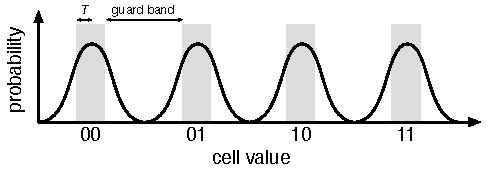
\includegraphics[scale=0.8]{figs/mlc-precise.pdf}
        \caption{Precise MLC}
        \label{approxstorage:fig:mlc-precise}
    \end{subfigure}
    \begin{subfigure}{0.5\columnwidth}
        \centering
        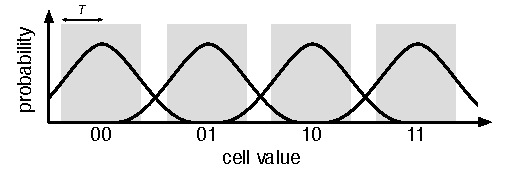
\includegraphics[scale=0.8]{figs/mlc-approx.pdf}
        \caption{Approximate MLC}
        \label{approxstorage:fig:mlc-approx}
    \end{subfigure}
    \caption{
        The range of analog values in a precise (a) and approximate (b) four-level cell. The shaded areas are
        the target regions for writes to each level (the parameter $T$ is half
        the width of a target region). Unshaded areas are
        \emph{guard bands}. The curves show the probability of reading a given
        analog value after writing one of the levels. Approximate  MLCs
        decrease guard bands so the probability distributions overlap.
    }
    \label{approxstorage:fig:mlc}
\end{figure}

PCM and other solid-state memories
work by storing an analog value---resistance, in PCM's case---and quantizing it to expose digital
storage. In multi-level cell (MLC) configurations, each cell stores
multiple bits. For \emph{precise} storage in MLC memory,
there is a trade-off between access cost and density: a larger number
of levels per cell requires more time and energy to access.
Furthermore, protections against analog sources of error like drift can consume
significant error correction overhead~\cite{drifttolerant}.
But, where perfect storage fidelity is not required,
performance and density can be improved beyond what is possible under
strict precision constraints.

An \emph{approximate MLC} configuration relaxes the strict precision
constraints on iterative MLC writes to improve their performance and energy
efficiency. Correspondingly, approximate MLC writes allow for denser cells
under fixed energy or performance budgets. Since PCM's write speed is expected
to be substantially slower than DRAM's, accelerating writes is critical to
realizing PCM as a main-memory technology~\cite{pcm-dram-alt}.
Reducing the energy
spent on writes conserves battery power in mobile devices, where
solid-state storage is commonplace.

Our approach to approximate MLC memory exploits the underlying
analog medium used to implement digital storage. Analog reads and
writes are inherently imprecise, so MLCs must incorporate \emph{guard
bands} that account for this imprecision and prevent storage errors.
These guard bands lead to tighter tolerances on target values, which in turn limit
the achievable write performance.
Approximate MLCs reduce or eliminate guard bands to speed up
iterative writes at the cost of occasional errors.
Figure~\ref{approxstorage:fig:mlc} illustrates this idea.

\subsection{Multi-Level Cell Model}
\label{approxstorage:sec:mlcmodel}

\begin{figure}
    \centering
    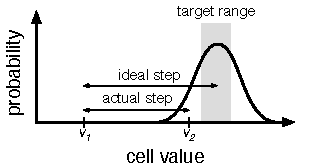
\includegraphics[scale=0.9]{figs/mlc-step}
    \caption{
        A single step in an iterative program-and-verify write. The value
        starts at $v_1$ and takes a step. The curve shows the probability
        distribution from which the ending value, $v_2$, is drawn. Here, since
        $v_2$ lies outside the target range, another step must be taken.
    }
    \label{approxstorage:fig:mlc-step}
\end{figure}

The basis for MLC storage is an underlying analog value (e.g., resistance for
PCM or charge for Flash).
We consider this value to be
continuous: while the memory quantizes the value to expose digital
storage externally, the internal value is conceptually
a real number between 0 and 1.\footnote{At small feature sizes, quantum effects may
cause values to appear discrete rather than
continuous. We do not consider these effects here.}
To implement
digital storage, the cell has $n$ discrete \emph{levels}, which are
internal analog-domain values corresponding to
external digital-domain values. As a simplification, we
assume that the levels are evenly distributed so that each level is
the center of an equally-sized, non-overlapping band of values: the
first level is $\frac{1}{2n}$, the second is $\frac{3}{2n}$, and so
on. In practice, values can be distributed exponentially, rather
    than linearly, in a cell's resistance range~\cite{mlcibm,partialreset}; in this case, the abstract value space corresponds
to the logarithm of the resistance. A cell with $n=2$ levels is
called a single-level cell (SLC) and any design with $n
> 2$ levels is a multi-level cell (MLC).

Writes and reads to the analog substrate are imperfect. A write
pulse, rather than adjusting the resistance by a precise amount,
changes it according to a probability distribution. During
reads, material nondeterminism causes the recovered value to differ
slightly from the value originally stored and, over time, the stored
value can change due to drift~\cite{wdddmlcpcm}.
Traditional (fully precise) cells are designed to minimize the
likelihood that write imprecision, read noise, or drift cause storage
errors in the digital domain. That is, given any digital value, a
write followed by a read recovers the same digital value with
high probability. In approximate storage, the goal is to increase
density or performance at the cost of occasional digital-domain
storage errors.

Put more formally, let $v$ be a cell's internal analog value. A
write operation for a digital value $d$ first determines
$l_d$, the value level corresponding to
$d$. Ideally, the write operation would set $v = l_d$ precisely.
Realistically, it sets $v$ to $w(l_d)$ where $w$ is an error
function introducing perturbations from the ideal analog value.
Similarly, a read operation recovers a perturbed analog value $r(v)$ and
quantizes it to obtain a digital output.

The number of levels, $n$, and the access error functions, $w$ and
$r$, determine the performance, density, and reliability of the cell.
Current designs trade off performance
for density---a dense cell with many levels requires tighter error
functions and is slower than sparser cells. Approximate
storage cells trade off the third dimension, reliability, to gain in
performance, density, or both.

\paragraph{Write error function}

A single programming pulse typically has poor
precision due to process variation and nondeterministic material
behavior. As a result, MLC designs for both Flash and PCM adopt iterative
program-and-verify (P\&V) mechanisms~\cite{morphablepcm,mlcflash}.
In PCM, each P\&V iteration adjusts the cell's resistance and then reads it
back to check whether the
correct value was achieved.
The process continues until an acceptable resistance value has been set.
To model the latency and error characteristics of iterative writes, we
consider the effect of each step to be drawn from a normal
distribution. The write mechanism determines the ideal pulse size but
applies that pulse with some error added.
Figure~\ref{approxstorage:fig:mlc-step} illustrates one iteration in this process.

Two parameters control the operation of the P\&V write algorithm.
First, iteration terminates when the stored value is within a
threshold distance $T$ from the target value. 
Setting $T < \frac{1}{2n}$ as in Figure~\ref{approxstorage:fig:mlc} provides \emph{guard bands} between the
levels to account for read error. The value of $T$ dictates the probability
that a read error will occur.
Second, the variance of
the normal distribution governing the effect of each pulse is modeled
as a constant proportion, $P$, of the intended step size. These parameters
determine the average number of iterations required to write the cell.

\begin{figure}
    \begin{center}
    \begin{minipage}{2in}
    \begin{lstlisting}[mathescape]
def $w$($v_t$):
  $v$ = 0
  while $|v_t - r(v)| > T$:
    size = $v_t - v$
    $v$ += $N(\mathrm{size}, P \cdot \mathrm{size})$
  return $v$
\end{lstlisting}
    \end{minipage}
    \end{center}
    \caption{
        Pseudocode for the write error function, $w$, in PCM
        cells.
        Here, $N(\mu, \sigma^2)$ is a normally distributed random
        variable
        with average $\mu$ and variance
        $\sigma^2$. The parameter $T$ controls the termination
        criterion and $P$ reflects the precision of each write pulse.
    }
    \label{approxstorage:fig:pcode-pcm}
\end{figure}

Figure~\ref{approxstorage:fig:pcode-pcm} shows the pseudocode for
writes, which resembles the PCM programming feedback
control loop of Pantazi et al.~\cite{mlcmodelchar}.
Section~\ref{approxstorage:sec:errorparams} describes our methodology for
calibrating the algorithm's parameters to reflect realistic PCM
systems.

Each constituent write pulse in an PCM write can either increase or decrease
resistance~\cite{mlcprogalgo,mlcibm,mlcmodelchar}.
Flash write pulses, in contrast, are unidirectional, so writes
must be more conservative to avoid costly RESET operations
in the case of overprogramming~\cite{ispp}.

\paragraph{Read error function}

Reading from a storage cell is also imprecise. PCM
cells are subject to both \emph{noise}, random variation in the stored value,
and \emph{drift}, a gradual unidirectional
shift~\cite{mlcpcmreliability}. We reuse the model and parameters of
Yeo et al.~\cite{wdddmlcpcm}. Namely, the sensed
analog value $r(v)$ is related to the written value $v$ as
$r(v) = v + \log_{10} t \cdot N(\mu_r, \sigma_r^2)$
where $t$ is the time, in seconds, elapsed since the cell was written.
The parameters $\mu_r$ and $\sigma_r$ are the mean and standard
deviation of the error effect respectively.

The same error function, with $t$ equal to the duration of a write step,
is used to model errors during the verification step of the write
process. We use $t = 250~\mathrm{ns}$~\cite{writecancel,improvingwrites} for
this case.

\paragraph{Read quantization}

A read operation must determine the digital value corresponding to the
analog value $r(v)$. We assume reads based on a successive
approximation analog-to-digital converter (ADC), which has been proposed for PCM
systems that can vary their level count~\cite{morphablepcm}. The
latency for a successive approximation ADC is linear in the number of
bits (i.e., $\log n$).

\paragraph{Model simplifications}

While this model is more detailed than some recent work, which has used simple
closed-form probability distributions to describe program-and-verify
writes~\cite{improvingwrites,writecancel}, it necessarily makes some
simplifications over the full complexity of the physics underlying PCM.

For simplicity, our model does not incorporate differential writes, a
technique that would allow a write to begin without an initial
RESET pulse~\cite{improvingwrites}. The write algorithm also does not
incorporate the detection of hard failures, which is typically
accomplished by timing out after a certain number of
iterations~\cite{mlcflash}. Hard failure detection is orthogonal to
the approximate MLC technique.

We measure write performance improvement in terms of the number of
iterations per write. While some MLC write techniques use different
durations for differently sized pulses~\cite{mlcmodelchar,partialreset,mlcwritestrategies}, we expect the
pulses to have approximately the same average time in aggregate.
Previous work, for example, has assumed that each step takes
250~nanoseconds~\cite{writecancel,improvingwrites}.
Furthermore, since our evaluation focuses on performance and energy, we do not
model any potential lifetime benefits afforded by the technique's reduction in
write pulses.

Finally, our model assumes for simplicity that the value range has
uniform guard band sizes: in terms of our model, the threshold $T$ is
constant among levels.
Asymmetric
guard bands could exploit the fact that drift is unidirectional.
This optimization is orthogonal to the approximate MLC technique,
which simply decreases the size of guard bands relative to their
nominal size.

\subsection{Encoding Values to Minimize Error}
\label{approxstorage:sec:coding}

MLC systems typically divide the bits from a single cell among different
memory pages~\cite{mlcflash}.
Using this technique, some pages consist of high-order bits from many cells
while other pages consist entirely of low-order bits. In approximate MLCs,
low-order bits are the least reliable. So this traditional strategy would lead
to pages with uniformly poor accuracy.
Here, we use a different approach in
order to represent all approximate values with acceptable accuracy.

If each cell has $n$ levels, then individual cells can each
represent $\log n$ bits. If a program needs to store $\log n$-bit
numbers, then the error characteristics of a single cell are
advantageous: a single-level
error---when the cell stores $l-1$ or $l+1$ after attempting to write
$l$---corresponds to a integer error of $1$ in the stored value.

\begin{figure}
    \begin{subfigure}{0.5\columnwidth}
        \centering
        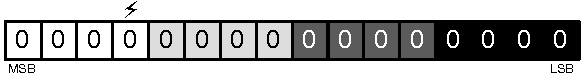
\includegraphics[scale=0.65]{figs/coding-chunk}
        \caption{Concatenation code}
        \label{approxstorage:fig:coding-chunk}
    \end{subfigure}
    \begin{subfigure}{0.5\columnwidth}
        \centering
        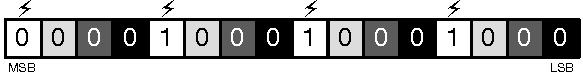
\includegraphics[scale=0.65]{figs/coding-stripe}
        \caption{Striping code}
        \label{approxstorage:fig:coding-stripe}
    \end{subfigure}
    \caption{
        Two codes for storing 16-bit numbers in four
        4-bit cells. Each color indicates a different cell.
        A single-level error leads to a bit flip in the indicated
        position.
        In (a), this is the lowest-order bit in the white cell.
        In (b), the white cell holds the binary value 0111, which is one level
        away from 1000.
    }
\end{figure}

But we also need to combine multiple cells to store larger numbers.
We consider two approaches. Concatenation
(Figure~\ref{approxstorage:fig:coding-chunk}) appends the bits from the
constituent cells to form each word. Striping
(Figure~\ref{approxstorage:fig:coding-stripe}) interleaves the cells so that the highest-order
bits of each cell all map to the highest-order bits of the word.

An ideal code would make errors in high bits rare while allowing more errors
in the low bits of a word. With the straightforward concatenation code, however,
a single-level error can cause a high-order bit flip: the word's $\log n$-th
most significant bit is the \emph{least} significant bit in its cell.
The striping code mitigates high-bit errors but does not prevent them. In the
example shown in Figure~\ref{approxstorage:fig:coding-stripe}, the white cell stores the
value 0111, so a single-level error can change its value to 1000. This error
causes a bit flip in the word's most significant bit.
(Gray coding, which some current MLC systems use~\cite{improvingwrites}, does
not address this problem: single-level errors are as likely to cause flips in
high-order bits as in low-order bits.)
We evaluate both approaches in
Section~\ref{approxstorage:sec:results} and find, as expected, that the striping code
mitigates errors most effectively.


\subsubsection{Defining an Optimal Code}

While the above bit-striping approach works well and is straightforward to
implement, it is not necessarily \emph{optimal:} there may exist other
coding schemes that further mitigate error.
Better codes have the potential to benefit any approximate-computing
technique that uses analog and multi-level substrates: not only storage but
also networking and communication channels.
Future work should explore strategies for deriving error-optimal codes.

As a first step in this direction, this section formalizes the notion of
error-minimizing, multi-level codes.
The two simple codes discussed above are points in a large space of possible
codes.
We also define the average error of a code as a way to quantify the code's error-mitigating
power.


Codes in this setting represent $b$-bit numbers (i.e., the first $2^b$ integers) using digits drawn from an alphabet of $n$ symbols. So a codeword $w = \langle v_1,
v_2, \dots, v_{b/\log n} \rangle$ is a vector of numbers $0 \le v < n$
where $n$ is the number of levels per cell. Assuming $n$ is a power of
two whose base divides $b$, there are $n ^ {b / \log n} = 2 ^ b$
codewords, so a code is bijection between the first $2^b$ integers and
the $2^b$ codewords.

Let the distance $d(w, w')$ between two codewords be the $l_1$ norm,
or the city block distance between the two vectors. We assume that the analog
medium confuses words with a smaller distance between them more often than
more distant words. Specifically, the probability that $w$ is written and $w'$ is subsequently recovered is inversely proportional to $d(w, w')$.

A \emph{code} is a function $c$ where $c(i)$ is the codeword that
represents the integer $i$. (The domain of $c$ is the integers $0 \le i <
2^b$.) The inverse, $c^{-1}(w)$, decodes a vector to the represented integer.

Let $A(w)$ be the random process that introduces these analog storage or
transmission errors into a codeword.
The overall average error of a code $c$ is:
%
$$\mathrm{E}\!\left[ |i - c^{-1}(A(c(i)))| \right]$$
%
An optimal code is one that minimizes this expected value when $i$
is drawn from a
uniform distribution (or some other sensible distribution).

An exhaustive search for the optimal code by this definition would be
intractable: there are $2^b!$ possible codes for $b$-bit numbers.
Recent work~\cite{holcomb-wacas} has used a constraint formulation to search a
subset of codes that reorder bits, but more sophisticated schemes
may exist that nonetheless have practical circuit-level implementations.
Future work should develop search strategies for low-error codes in
the enormous space of possible mappings.


\subsection{Memory Interface}

MLC blocks can be made precise or approximate by adjusting the target threshold of write
operations. For this reason, the memory array must know which threshold value
to use for each write operation. Rather than storing the precision level as
metadata for each block of memory, we encode that information in the operation itself by extending the memory interface to include
precision flags as described in Section~\ref{approxstorage:sec:idea}. This approach, aside
from eliminating metadata space overhead, eliminates the need for a metadata
read on the critical path for writes.

Read operations are identical for approximate and precise memory, so the
precision flag in read operations goes unused. A different approximate MLC
design could adjust the cell density of approximate memory; in this case, the
precision flag would control the bit width of the ADC
circuitry~\cite{morphablepcm}.

\paragraph{Overheads}

Since no metadata is used to control cells' precision, this scheme carries no
space overhead. However, at least one additional bit is necessary in each read
and write request on the memory interface to indicate the operation's
precision. If multiple threshold values are provided to support varying precision
levels, multiple bits will be needed. Additional circuitry may also be
necessary to permit a tunable threshold value during cell writes. Our performance
evaluation, in Section~\ref{approxstorage:sec:eval}, does not quantify these circuit area overheads.

\section{Using Failed Memory Cells}
\label{approxstorage:sec:recycling}

PCM, along with Flash and other upcoming memory technologies, suffers from cell
failures during a device's deployment---it ``wears out.'' Thus, techniques for hiding failures from
software are critical to providing a useful lifespan for a
memory~\cite{pcm-dram-alt}.
These techniques typically abandon portions of memory containing
uncorrectable failures and use only failure-free blocks~\cite{ecp,payg,safer}.
By employing otherwise-unusable failed blocks to
store \emph{approximate} data, it is possible to extend the
lifetime of an array as long as sufficient intact capacity remains to
store the application's \emph{precise} data.

The key idea is to use blocks with exhausted
error-correction resources to store approximate data. Previous work on
approximate storage in DRAM~\cite{flikker} and SRAM~\cite{truffle} has examined
\emph{soft} errors, which occur randomly in time and space.
If approximate data is stored in PCM blocks with failed cells, on the other
hand, errors will be
\emph{persistent}. That is, a value stored in a particular failed
block will consistently exhibit bit errors in the same positions.
We can
exploit the awareness of failure positions to provide more effective
error correction via \emph{bit priorities}.

\subsection{Prioritized Bit Correction}
\label{approxstorage:sec:bitprior}

In an error model incorporating
stuck-at failures, we can use error correction to concentrate
failures
where they are likely to do the least harm. For example, when storing
a floating-point number, a bit error is least significant when it
occurs in the low bits of the mantissa and most detrimental when it
occurs in the high bits of the exponent or the sign bit. In a uniform-probability
error model, errors in each location are equally likely, while a
deterministic-failure model affords the opportunity to protect
a value's most important bits.

A correction scheme like error-correcting pointers (ECP)~\cite{ecp} marks failed bits in a
block. Each block has limited correction resources; for example,
when the technique is provisioned to correct two bits per block (ECP$_2$),
a block becomes unusable for precise storage when three
bits fail. For approximate storage, we
can use ECP to correct the bits that appear in high-order positions
within words and leave the lowest-order failed bits uncorrected. As
more failures appear in this block, only the least-harmful stuck bits will
remain uncorrected.

\subsection{Memory Interface}
\label{approxstorage:sec:recycling-interface}

A memory module supporting failed-block recycling determines which blocks are
approximate and which may be used for precise storage. Unlike with the
approximate MLC technique (Section~\ref{approxstorage:sec:amlc}), software has no control
over blocks' precision state. To permit safe allocation of approximate and
precise data, the memory must inform software of the locations of approximate
(i.e., failed) blocks.

When the memory module is new, all blocks are precise. When the first
uncorrectable failure occurs in a block, the memory issues an interrupt
and indicates the failed block.
This is similar to other systems that use page remapping to retire failed
segments of memory~\cite{durable-pcm-mm,drm}.
The OS adds the
block to a pool of approximate blocks. Memory allocators consult this set of
approximate blocks when laying out data in the memory. While approximate data
can be stored in any block, precise data must be allocated in memory without
failures. Eventually, when too many blocks are approximate, the allocator will
not be able to find space for all precise data---at this point, the memory
module must be replaced.

To provide traditional error correction for precise data, the memory system must be
able to detect hard failures after each write~\cite{ecp}. We reuse this
existing error detection support; the precision level of
the write operation (see Section~\ref{approxstorage:sec:idea}) determines the action taken
when a failure is detected. When a failure occurs during a precise write, the
module either constructs ECP entries for all failed bits if sufficient
entries are available or issues an interrupt otherwise. When a failure occurs
during an approximate write, no interrupt is issued. The memory silently
corrects as many errors as possible and leaves the remainder uncorrected.

To make bit prioritization work, the memory module needs information from
the software indicating which bits are most important. Software specifies this
using a value size associated with each approximate write as described in
Section~\ref{approxstorage:sec:idea}. The value size indicates the homogenous byte-width of
approximate values stored in the block. If a block represents part of an array
of double-precision floating point numbers, for example, the appropriate value
size is 8 bytes. This indicates to the memory that the bits at index $i$ where
$i \equiv 0 \bmod{64}$ are most important, followed by $1 \bmod{64}$, etc. When
a block experiences a new failure and the memory module must
choose which errors to correct, it masks the bit indices of
each failure to obtain the index modulo 64. It corrects the bits with the
lowest indices and leaves the remaining failures uncorrected.

This interface for controlling bit prioritization requires blocks to contain
homogeneously sized values. In our experience, this is a common case: many of
the applications we examined use approximate
\texttt{double[]} or \texttt{float[]} arrays that span many blocks.

\paragraph{Overheads}

Like the approximate MLC scheme, failed-block recycling requires additional
bits for each read and write operation in the memory interface.
Messages must contain a precision flag and, to enable bit priority, a value
size field.
The memory module must incorporate logic to select the highest-priority bits
to correct in an approximate block; however, this selection happens rarely
because it need only occur when new failures arise.
Finally, to correctly allocate new memory, the OS must maintain a pool of
failed blocks and avoid using them for precise storage.
This block tracking is analogous to the way that Flash translation
layers (FTLs) remap bad blocks.


\section{Evaluation}
\label{approxstorage:sec:eval}

Approximate storage trades off precision for performance, durability, and density.
To understand this trade-off in the context of real-world approximate data, we
simulate both of our techniques and examine their effects on the quality of
data sets and application outputs. As with previous work on approximate
computing~\cite{enerj,npu,perforation}, we use
application-specific metrics to quantify quality
degradation.

We first describe the main-memory and persistent-data benchmarks used in our
evaluation. We then detail the MLC model parameters that dictate performance
and error rates of the approximate MLC technique. Finally, we describe the
model for wear-out used in our evaluation of the failed-block recycling
technique.

\subsection{Applications}

We use two types of benchmarks in our evaluation: main-memory applications and
persistent data sets. The main-memory applications are Java programs annotated
using the EnerJ~\cite{enerj} approximation-aware type system, which marks some
data as approximate and leaves other data precise. The persistent-storage
benchmarks are static data sets that can be stored 100\% approximately.

For the main-memory applications, we adapt the annotated benchmarks
from the evaluation of EnerJ. An in-house simulator intercepts
loads and stores to collect access statistics and inject errors. The
applications are chosen from a broad range of domains for their tolerance to
imprecision. We examine a 3D triangle intersection kernel from a game engine
(\textsf{jmeint}), a ray tracing image renderer (\textsf{raytracer}), a visual
bar code recognizer for mobile phones (\textsf{zxing}), and five scientific
kernels from the SciMark2 benchmark suite (\textsf{fft}, \textsf{lu},
\textsf{mc}, \textsf{smm}, and \textsf{sor}).
For the benchmarks with vector or matrix
output, the error metric is the mean pointwise entry difference. For the
benchmarks with all-or-nothing output correctness, \textsf{jmeint} and
\textsf{zxing}, the metric is the proportion of correct decisions. For
\textsf{raytracer}, the metric is the mean pixel value difference.
The evaluation of EnerJ~\cite{enerj}
contains more details on the annotation and quality assessment of these
benchmarks.

For persistent storage, we examine four sets of approximate data. The first,
\textsf{sensorlog}, consists of a log of mobile-phone sensor readings from an
accelerometer, thermometer, photodetector, and hydrometer. The data is used in
a decision tree to infer the device's context, so our quality metric is the
accuracy of this prediction relative to a fully-precise data set.
The second, \textsf{image}, stores
a bitmap photograph as an array of integer RGB values. The quality metric is
the mean error of the pixel values.
The final two data sets, \textsf{svm} and \textsf{ann}, are trained
classifiers for handwritten digit recognition based on a support vector
machine and a feed-forward neural network. In both cases,
the classifiers were trained using standard algorithms on the ``pendigits''
data set from the UCI Machine Learning Repository~\cite{ucimlrepo}.
The data set consists of 3498 training samples and 7494 testing samples, each
of which comprises 16 features.
Then, the classifier
parameters (support vectors and neuron weights, respectively) are stored in
approximate memory.
The SVM uses 3024 support vectors; the NN is configured with a sigmoid
activation function, two hidden layers
of 128 neurons each, and a one-hot output layer of 10 neurons.
We measure the recognition accuracy of each classifier on
an unseen test data set relative to the accuracy of the precise classifier
(95\% for \textsf{svm} and 80\% for \textsf{ann}).
Unlike the main-memory applications, which consist of a mixture
of approximate and precise data,
the persistent data sets are entirely
approximate.

\subsection{MLC Model Parameters}
\label{approxstorage:sec:errorparams}

To assess our approximate MLC technique, we use the model described in
Section~\ref{approxstorage:sec:mlcmodel}. The abstract model has a number of parameters that
we need to select for the purposes of simulation. To set the parameters, we use
values from the literature on MLC PCM configurations. Since our
architecture-level model of iterative program-and-verify writes is original, we
infer its parameters by calibrating them to match typical write latencies and error
rates.

For a baseline (precise) MLC PCM cell, we need a configuration where
errors are improbable but not impossible. We choose a conservative
baseline raw bit error rate (RBER) of $10^{-8}$, which comports with
RBERs observed in Flash memory today~\cite{flasherror,flasherrors}.

We first select parameters for the read model in Section~\ref{approxstorage:sec:mlcmodel},
which incorporates the probabilistic effects of read noise and drift.
% for level 1, mu = 0.02 and sigma = 0.4 * mu
% but this is for a value range from 3.0 to 6.0, so we divide mu by 3
% for our 0-1 range
For the parameters $\mu_r$ and $\sigma_r$, we use typical values from
Yeo et al.~\cite{wdddmlcpcm} normalized to our presumed 0.0--1.0 value
range. Specifically, for PCM, we choose $\mu_r = 0.0067$ and $\sigma_r
= 0.0027$. Since the read model incorporates drift, it is sensitive to
the retention time between writes and reads. Retention time can be
short in a main-memory deployment and much longer when PCM is
used for persistent storage.  As an intermediate value, we consider
retention for $t = 10^{5}$ seconds, or slightly more than one day.
Note that this retention time is pessimistic for the main-memory
case: in our experiments, every read experiences error as if it
occurred $10^5$ seconds after the preceding write. In real software,
the interval between writes and subsequent reads is typically much
lower.

We model a 4-level (2-bit) PCM cell. To calibrate the write model, we start from an average write
time of 3 cycles as suggested by Nirschl et
al.~\cite{mlcwritestrategies} and a target RBER of $10^{-8}$.
We need values for the parameters $T$ and $P$ that
match these characteristics. We choose our baseline threshold to be 20\%
of the largest threshold that leads to non-overlapping values
(i.e., $T = 0.025$); this leads to about 3 iterations per write.
Setting $P = 0.035$ leads to an error probability on the order of
$10^{-8}$ for a retention time of $10^5$ seconds.
% P = 0.035
% T = 0.2 * nominal
% error probability at this config is measured at 1.95e-8 (per day)

\subsection{Wear-Out Model}
\label{approxstorage:sec:wearmodel}

To evaluate the effect of using blocks with failed cells for approximate
storage, we simulate single-level PCM.
In single-level PCM,
bits become
stuck independently as their underlying cells fail.
With multi-level designs, in contrast, a single cell failure can cause
multiple bits to become stuck, so bit failures are not independent.
Assuming that the memory assigns bits from a given cell to distinct
pages~\cite{mlcflash} and that wear leveling randomly remaps pages,
failures nonetheless \emph{appear} independent in multi-level PCM.
So a multi-level
failure model would closely resemble our single-level model with an
accelerated failure rate.

We evaluate PCM with 2-bit error-correcting pointers (ECP)~\cite{ecp}.
While precise configurations of the ECP technique typically use 6-bit
correction, approximate storage can extend device lifetime without incurring as
much overhead as a fully precise configuration.
Approximate blocks also use the bit priority assignment mechanism from
Section~\ref{approxstorage:sec:bitprior}: where possible, ECP corrections are allocated to
higher-order bits within each value in the block.

To understand the occurrence of stuck bits in failed blocks,
we need a realistic model for the rate at which cells wear out over time.
To this end,
we simulate a PCM array for trillions of writes and
measure the distribution of cell failures among blocks.
The statistical simulator is adapted from Azevedo et al.~\cite{zombie} and
assumes an average PCM cell lifetime of $10^8$ writes (although
the \emph{first} failure occurs much earlier).
We use separate
workloads to simulate wear in a main-memory setting and in a persistent-storage
setting.

\paragraph{Main-memory wear}

\begin{figure}[t]
    \centering
    % GNUPLOT: LaTeX picture with Postscript
\begingroup
\sffamily \footnotesize
  \makeatletter
  \providecommand\color[2][]{%
    \GenericError{(gnuplot) \space\space\space\@spaces}{%
      Package color not loaded in conjunction with
      terminal option `colourtext'%
    }{See the gnuplot documentation for explanation.%
    }{Either use 'blacktext' in gnuplot or load the package
      color.sty in LaTeX.}%
    \renewcommand\color[2][]{}%
  }%
  \providecommand\includegraphics[2][]{%
    \GenericError{(gnuplot) \space\space\space\@spaces}{%
      Package graphicx or graphics not loaded%
    }{See the gnuplot documentation for explanation.%
    }{The gnuplot epslatex terminal needs graphicx.sty or graphics.sty.}%
    \renewcommand\includegraphics[2][]{}%
  }%
  \providecommand\rotatebox[2]{#2}%
  \@ifundefined{ifGPcolor}{%
    \newif\ifGPcolor
    \GPcolorfalse
  }{}%
  \@ifundefined{ifGPblacktext}{%
    \newif\ifGPblacktext
    \GPblacktexttrue
  }{}%
  % define a \g@addto@macro without @ in the name:
  \let\gplgaddtomacro\g@addto@macro
  % define empty templates for all commands taking text:
  \gdef\gplbacktext{}%
  \gdef\gplfronttext{}%
  \makeatother
  \ifGPblacktext
    % no textcolor at all
    \def\colorrgb#1{}%
    \def\colorgray#1{}%
  \else
    % gray or color?
    \ifGPcolor
      \def\colorrgb#1{\color[rgb]{#1}}%
      \def\colorgray#1{\color[gray]{#1}}%
      \expandafter\def\csname LTw\endcsname{\color{white}}%
      \expandafter\def\csname LTb\endcsname{\color{black}}%
      \expandafter\def\csname LTa\endcsname{\color{black}}%
      \expandafter\def\csname LT0\endcsname{\color[rgb]{1,0,0}}%
      \expandafter\def\csname LT1\endcsname{\color[rgb]{0,1,0}}%
      \expandafter\def\csname LT2\endcsname{\color[rgb]{0,0,1}}%
      \expandafter\def\csname LT3\endcsname{\color[rgb]{1,0,1}}%
      \expandafter\def\csname LT4\endcsname{\color[rgb]{0,1,1}}%
      \expandafter\def\csname LT5\endcsname{\color[rgb]{1,1,0}}%
      \expandafter\def\csname LT6\endcsname{\color[rgb]{0,0,0}}%
      \expandafter\def\csname LT7\endcsname{\color[rgb]{1,0.3,0}}%
      \expandafter\def\csname LT8\endcsname{\color[rgb]{0.5,0.5,0.5}}%
    \else
      % gray
      \def\colorrgb#1{\color{black}}%
      \def\colorgray#1{\color[gray]{#1}}%
      \expandafter\def\csname LTw\endcsname{\color{white}}%
      \expandafter\def\csname LTb\endcsname{\color{black}}%
      \expandafter\def\csname LTa\endcsname{\color{black}}%
      \expandafter\def\csname LT0\endcsname{\color{black}}%
      \expandafter\def\csname LT1\endcsname{\color{black}}%
      \expandafter\def\csname LT2\endcsname{\color{black}}%
      \expandafter\def\csname LT3\endcsname{\color{black}}%
      \expandafter\def\csname LT4\endcsname{\color{black}}%
      \expandafter\def\csname LT5\endcsname{\color{black}}%
      \expandafter\def\csname LT6\endcsname{\color{black}}%
      \expandafter\def\csname LT7\endcsname{\color{black}}%
      \expandafter\def\csname LT8\endcsname{\color{black}}%
    \fi
  \fi
  \setlength{\unitlength}{0.0500bp}%
  \begin{picture}(4030.00,2880.00)%
    \gplgaddtomacro\gplbacktext{%
      \csname LTb\endcsname%
      \put(726,638){\makebox(0,0)[r]{\strut{} 0}}%
      \put(726,1132){\makebox(0,0)[r]{\strut{} 0.1}}%
      \put(726,1627){\makebox(0,0)[r]{\strut{} 0.2}}%
      \put(726,2121){\makebox(0,0)[r]{\strut{} 0.3}}%
      \put(726,2615){\makebox(0,0)[r]{\strut{} 0.4}}%
      \put(1043,418){\makebox(0,0){\strut{} 1}}%
      \put(1351,418){\makebox(0,0){\strut{} 2}}%
      \put(1660,418){\makebox(0,0){\strut{} 3}}%
      \put(1968,418){\makebox(0,0){\strut{} 4}}%
      \put(2276,418){\makebox(0,0){\strut{} 5}}%
      \put(2585,418){\makebox(0,0){\strut{} 6}}%
      \put(2893,418){\makebox(0,0){\strut{} 7}}%
      \put(3201,418){\makebox(0,0){\strut{} 8}}%
      \put(3510,418){\makebox(0,0){\strut{} 9}}%
      \put(272,1626){\rotatebox{-270}{\makebox(0,0){\strut{}frequency}}}%
      \put(2245,154){\makebox(0,0){\strut{}uncorrectable failures per block}}%
    }%
    \gplgaddtomacro\gplfronttext{%
    }%
    \gplbacktext
    \put(0,0){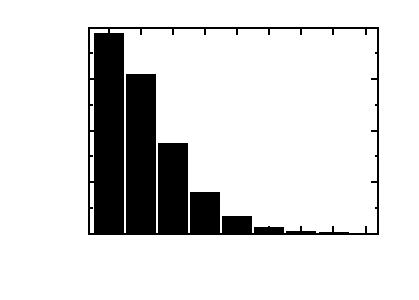
\includegraphics{plots/err_hist}}%
    \gplfronttext
  \end{picture}%
\endgroup

    \caption{
        Distribution of uncorrectable cell failures using ECP$_2$ among
        512-bit blocks
        after the entire memory has been overwritten
        $3.2 \times 10^{7}$ times under the main-memory wear model. (At this
        stage, half of the blocks have at least one uncorrectable failure.)
    }
    \label{approxstorage:fig:hist}
\end{figure}

To model wear in main-memory PCM deployments, we simulate the above suite of main-memory
applications and gather statistics about their memory access patterns,
including the relative size of each program's approximate vs.~precise
data and the frequency of writes to each type of memory. We then take
the harmonic mean of these statistics to create an aggregate workload
consisting of the entire suite. We run a statistical PCM
simulation based on these application characteristics, during which
all blocks start out precise. When a block experiences
its first uncorrectable cell failure, it is moved to the approximate
pool. Failed blocks
continue to be written and experience additional bit failures because they store
approximate data. Periodically, we record the amount of
memory that remains precise along with the distribution of failures
among the approximate blocks.
We simulate each application under these measured failure conditions.

As an example, Figure~\ref{approxstorage:fig:hist} depicts the error rate distribution for the
wear stage at which 50\% of the memory's blocks have at least one failure that
is uncorrectable using ECP$_2$---i.e.,
half the blocks are approximate. In this stage,
most the of the blocks have only a few uncorrectable failures: 39\% of the
approximate blocks have exactly one such failure and only 1.7\% have
six or more.



\paragraph{Persistent-storage wear} For our persistent-storage data sets, all
data is approximate. So we simulate writes uniformly across all of
memory, both failed and fully-precise. This corresponds to a usage scenario in
which the PCM array is entirely dedicated to persistent storage---no hybrid
transient/persistent storage is assumed. As with the main-memory wear model, we
periodically snapshot the distribution of errors among all blocks and use these
to inject bit errors into stored data.


\section{Results}
\label{approxstorage:sec:results}

We evaluate both sets of benchmarks under each of our two approximate storage
techniques.
We first measure the approximate MLC mechanism.

\subsection{Approximate MLC Memory}

In our approximate MLC experiments, we map all approximate data to simulated
arrays of two-bit PCM cells. We run each benchmark multiple times with
differing threshold ($T$) parameters. We use $T$ values between 20\%
and 90\% of the maximum threshold (i.e., the threshold that eliminates
guard bands altogether).
For each threshold, we measure the
average number of iterations required to write a random value.
This yields an application-independent metric that is
directly proportional to write latency (i.e., inversely
proportional to performance). Configurations with fewer iterations per write
are faster but cause more errors. So, for each application, the optimal
configuration is the one that decreases write iterations the most while
sacrificing as little output quality as possible.
Faster writes help close PCM's performance gap with DRAM in the main-memory
case and improve write bandwidth in the persistent-data
case~\cite{pcm-dram-alt,flash-retention-relax}.

\paragraph{Approximate main memory}

\begin{figure}
    \begin{subfigure}[b]{0.5\columnwidth}
        \centering
        % GNUPLOT: LaTeX picture with Postscript
\begingroup
\sffamily \footnotesize
  \makeatletter
  \providecommand\color[2][]{%
    \GenericError{(gnuplot) \space\space\space\@spaces}{%
      Package color not loaded in conjunction with
      terminal option `colourtext'%
    }{See the gnuplot documentation for explanation.%
    }{Either use 'blacktext' in gnuplot or load the package
      color.sty in LaTeX.}%
    \renewcommand\color[2][]{}%
  }%
  \providecommand\includegraphics[2][]{%
    \GenericError{(gnuplot) \space\space\space\@spaces}{%
      Package graphicx or graphics not loaded%
    }{See the gnuplot documentation for explanation.%
    }{The gnuplot epslatex terminal needs graphicx.sty or graphics.sty.}%
    \renewcommand\includegraphics[2][]{}%
  }%
  \providecommand\rotatebox[2]{#2}%
  \@ifundefined{ifGPcolor}{%
    \newif\ifGPcolor
    \GPcolorfalse
  }{}%
  \@ifundefined{ifGPblacktext}{%
    \newif\ifGPblacktext
    \GPblacktexttrue
  }{}%
  % define a \g@addto@macro without @ in the name:
  \let\gplgaddtomacro\g@addto@macro
  % define empty templates for all commands taking text:
  \gdef\gplbacktext{}%
  \gdef\gplfronttext{}%
  \makeatother
  \ifGPblacktext
    % no textcolor at all
    \def\colorrgb#1{}%
    \def\colorgray#1{}%
  \else
    % gray or color?
    \ifGPcolor
      \def\colorrgb#1{\color[rgb]{#1}}%
      \def\colorgray#1{\color[gray]{#1}}%
      \expandafter\def\csname LTw\endcsname{\color{white}}%
      \expandafter\def\csname LTb\endcsname{\color{black}}%
      \expandafter\def\csname LTa\endcsname{\color{black}}%
      \expandafter\def\csname LT0\endcsname{\color[rgb]{1,0,0}}%
      \expandafter\def\csname LT1\endcsname{\color[rgb]{0,1,0}}%
      \expandafter\def\csname LT2\endcsname{\color[rgb]{0,0,1}}%
      \expandafter\def\csname LT3\endcsname{\color[rgb]{1,0,1}}%
      \expandafter\def\csname LT4\endcsname{\color[rgb]{0,1,1}}%
      \expandafter\def\csname LT5\endcsname{\color[rgb]{1,1,0}}%
      \expandafter\def\csname LT6\endcsname{\color[rgb]{0,0,0}}%
      \expandafter\def\csname LT7\endcsname{\color[rgb]{1,0.3,0}}%
      \expandafter\def\csname LT8\endcsname{\color[rgb]{0.5,0.5,0.5}}%
    \else
      % gray
      \def\colorrgb#1{\color{black}}%
      \def\colorgray#1{\color[gray]{#1}}%
      \expandafter\def\csname LTw\endcsname{\color{white}}%
      \expandafter\def\csname LTb\endcsname{\color{black}}%
      \expandafter\def\csname LTa\endcsname{\color{black}}%
      \expandafter\def\csname LT0\endcsname{\color{black}}%
      \expandafter\def\csname LT1\endcsname{\color{black}}%
      \expandafter\def\csname LT2\endcsname{\color{black}}%
      \expandafter\def\csname LT3\endcsname{\color{black}}%
      \expandafter\def\csname LT4\endcsname{\color{black}}%
      \expandafter\def\csname LT5\endcsname{\color{black}}%
      \expandafter\def\csname LT6\endcsname{\color{black}}%
      \expandafter\def\csname LT7\endcsname{\color{black}}%
      \expandafter\def\csname LT8\endcsname{\color{black}}%
    \fi
  \fi
  \setlength{\unitlength}{0.0500bp}%
  \begin{picture}(4030.00,3628.00)%
    \gplgaddtomacro\gplbacktext{%
      \csname LTb\endcsname%
      \put(858,462){\makebox(0,0)[r]{\strut{}0\%}}%
      \put(858,886){\makebox(0,0)[r]{\strut{}20\%}}%
      \put(858,1310){\makebox(0,0)[r]{\strut{}40\%}}%
      \put(858,1734){\makebox(0,0)[r]{\strut{}60\%}}%
      \put(858,2158){\makebox(0,0)[r]{\strut{}80\%}}%
      \put(858,2582){\makebox(0,0)[r]{\strut{}100\%}}%
      \put(3324,242){\makebox(0,0){\strut{} 1.6}}%
      \put(2996,242){\makebox(0,0){\strut{} 1.8}}%
      \put(2669,242){\makebox(0,0){\strut{} 2}}%
      \put(2341,242){\makebox(0,0){\strut{} 2.2}}%
      \put(2014,242){\makebox(0,0){\strut{} 2.4}}%
      \put(1687,242){\makebox(0,0){\strut{} 2.6}}%
      \put(1359,242){\makebox(0,0){\strut{} 2.8}}%
      \put(1032,242){\makebox(0,0){\strut{} 3}}%
      \put(286,1522){\rotatebox{-270}{\makebox(0,0){\strut{}output quality loss}}}%
      \put(2311,22){\makebox(0,0){\strut{}average write steps}}%
    }%
    \gplgaddtomacro\gplfronttext{%
      \csname LTb\endcsname%
      \put(1263,3455){\makebox(0,0)[r]{\strut{}fft}}%
      \csname LTb\endcsname%
      \put(1263,3235){\makebox(0,0)[r]{\strut{}zxing}}%
      \csname LTb\endcsname%
      \put(1263,3015){\makebox(0,0)[r]{\strut{}jmeint}}%
      \csname LTb\endcsname%
      \put(1263,2795){\makebox(0,0)[r]{\strut{}lu}}%
      \csname LTb\endcsname%
      \put(2778,3455){\makebox(0,0)[r]{\strut{}smm}}%
      \csname LTb\endcsname%
      \put(2778,3235){\makebox(0,0)[r]{\strut{}mc}}%
      \csname LTb\endcsname%
      \put(2778,3015){\makebox(0,0)[r]{\strut{}raytracer}}%
      \csname LTb\endcsname%
      \put(2778,2795){\makebox(0,0)[r]{\strut{}sor}}%
    }%
    \gplbacktext
    \put(0,0){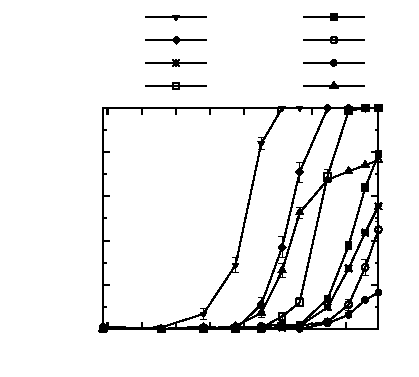
\includegraphics{plots/qos_mlc-stripe}}%
    \gplfronttext
  \end{picture}%
\endgroup

        \caption{
            Main-memory applications with approximate MLC.
        }
        \label{approxstorage:fig:qos-mlc}
    \end{subfigure}
    \begin{subfigure}[b]{0.5\columnwidth}
        \centering
        % GNUPLOT: LaTeX picture with Postscript
\begingroup
\sffamily \footnotesize
  \makeatletter
  \providecommand\color[2][]{%
    \GenericError{(gnuplot) \space\space\space\@spaces}{%
      Package color not loaded in conjunction with
      terminal option `colourtext'%
    }{See the gnuplot documentation for explanation.%
    }{Either use 'blacktext' in gnuplot or load the package
      color.sty in LaTeX.}%
    \renewcommand\color[2][]{}%
  }%
  \providecommand\includegraphics[2][]{%
    \GenericError{(gnuplot) \space\space\space\@spaces}{%
      Package graphicx or graphics not loaded%
    }{See the gnuplot documentation for explanation.%
    }{The gnuplot epslatex terminal needs graphicx.sty or graphics.sty.}%
    \renewcommand\includegraphics[2][]{}%
  }%
  \providecommand\rotatebox[2]{#2}%
  \@ifundefined{ifGPcolor}{%
    \newif\ifGPcolor
    \GPcolorfalse
  }{}%
  \@ifundefined{ifGPblacktext}{%
    \newif\ifGPblacktext
    \GPblacktexttrue
  }{}%
  % define a \g@addto@macro without @ in the name:
  \let\gplgaddtomacro\g@addto@macro
  % define empty templates for all commands taking text:
  \gdef\gplbacktext{}%
  \gdef\gplfronttext{}%
  \makeatother
  \ifGPblacktext
    % no textcolor at all
    \def\colorrgb#1{}%
    \def\colorgray#1{}%
  \else
    % gray or color?
    \ifGPcolor
      \def\colorrgb#1{\color[rgb]{#1}}%
      \def\colorgray#1{\color[gray]{#1}}%
      \expandafter\def\csname LTw\endcsname{\color{white}}%
      \expandafter\def\csname LTb\endcsname{\color{black}}%
      \expandafter\def\csname LTa\endcsname{\color{black}}%
      \expandafter\def\csname LT0\endcsname{\color[rgb]{1,0,0}}%
      \expandafter\def\csname LT1\endcsname{\color[rgb]{0,1,0}}%
      \expandafter\def\csname LT2\endcsname{\color[rgb]{0,0,1}}%
      \expandafter\def\csname LT3\endcsname{\color[rgb]{1,0,1}}%
      \expandafter\def\csname LT4\endcsname{\color[rgb]{0,1,1}}%
      \expandafter\def\csname LT5\endcsname{\color[rgb]{1,1,0}}%
      \expandafter\def\csname LT6\endcsname{\color[rgb]{0,0,0}}%
      \expandafter\def\csname LT7\endcsname{\color[rgb]{1,0.3,0}}%
      \expandafter\def\csname LT8\endcsname{\color[rgb]{0.5,0.5,0.5}}%
    \else
      % gray
      \def\colorrgb#1{\color{black}}%
      \def\colorgray#1{\color[gray]{#1}}%
      \expandafter\def\csname LTw\endcsname{\color{white}}%
      \expandafter\def\csname LTb\endcsname{\color{black}}%
      \expandafter\def\csname LTa\endcsname{\color{black}}%
      \expandafter\def\csname LT0\endcsname{\color{black}}%
      \expandafter\def\csname LT1\endcsname{\color{black}}%
      \expandafter\def\csname LT2\endcsname{\color{black}}%
      \expandafter\def\csname LT3\endcsname{\color{black}}%
      \expandafter\def\csname LT4\endcsname{\color{black}}%
      \expandafter\def\csname LT5\endcsname{\color{black}}%
      \expandafter\def\csname LT6\endcsname{\color{black}}%
      \expandafter\def\csname LT7\endcsname{\color{black}}%
      \expandafter\def\csname LT8\endcsname{\color{black}}%
    \fi
  \fi
  \setlength{\unitlength}{0.0500bp}%
  \begin{picture}(4030.00,3168.00)%
    \gplgaddtomacro\gplbacktext{%
      \csname LTb\endcsname%
      \put(858,462){\makebox(0,0)[r]{\strut{}0\%}}%
      \put(858,884){\makebox(0,0)[r]{\strut{}20\%}}%
      \put(858,1306){\makebox(0,0)[r]{\strut{}40\%}}%
      \put(858,1729){\makebox(0,0)[r]{\strut{}60\%}}%
      \put(858,2151){\makebox(0,0)[r]{\strut{}80\%}}%
      \put(858,2573){\makebox(0,0)[r]{\strut{}100\%}}%
      \put(3324,242){\makebox(0,0){\strut{} 1.6}}%
      \put(2996,242){\makebox(0,0){\strut{} 1.8}}%
      \put(2669,242){\makebox(0,0){\strut{} 2}}%
      \put(2341,242){\makebox(0,0){\strut{} 2.2}}%
      \put(2014,242){\makebox(0,0){\strut{} 2.4}}%
      \put(1687,242){\makebox(0,0){\strut{} 2.6}}%
      \put(1359,242){\makebox(0,0){\strut{} 2.8}}%
      \put(1032,242){\makebox(0,0){\strut{} 3}}%
      \put(286,1517){\rotatebox{-270}{\makebox(0,0){\strut{}output quality loss}}}%
      \put(2311,22){\makebox(0,0){\strut{}average write steps}}%
    }%
    \gplgaddtomacro\gplfronttext{%
      \csname LTb\endcsname%
      \put(1263,2995){\makebox(0,0)[r]{\strut{}ann}}%
      \csname LTb\endcsname%
      \put(1263,2775){\makebox(0,0)[r]{\strut{}sensorlog}}%
      \csname LTb\endcsname%
      \put(2778,2995){\makebox(0,0)[r]{\strut{}image}}%
      \csname LTb\endcsname%
      \put(2778,2775){\makebox(0,0)[r]{\strut{}svm}}%
    }%
    \gplbacktext
    \put(0,0){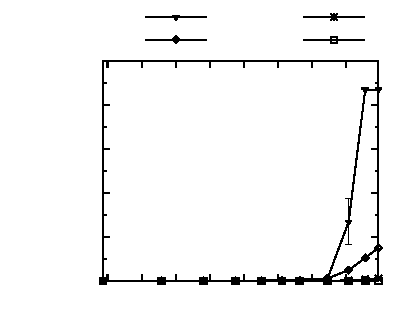
\includegraphics{plots/nv_qos_mlc-stripe}}%
    \gplfronttext
  \end{picture}%
\endgroup

        \caption{
            Persistent data sets with approximate MLC.
        }
        \label{approxstorage:fig:nv-qos-mlc}
    \end{subfigure}
    \caption{
        Output degradation for each benchmark using the approximate
        MLC technique.
        The horizontal
        axis shows the average number of iterations per write.
        The vertical axis is the output quality loss as
        defined by each application's quality metric.
        Quality loss is averaged over 100 executions in (a) and 10 in (b); the
        error bars show the standard error of the mean.
    }
\end{figure}

\begin{figure}
    \centering
    % GNUPLOT: LaTeX picture with Postscript
\begingroup
\sffamily \footnotesize
  \makeatletter
  \providecommand\color[2][]{%
    \GenericError{(gnuplot) \space\space\space\@spaces}{%
      Package color not loaded in conjunction with
      terminal option `colourtext'%
    }{See the gnuplot documentation for explanation.%
    }{Either use 'blacktext' in gnuplot or load the package
      color.sty in LaTeX.}%
    \renewcommand\color[2][]{}%
  }%
  \providecommand\includegraphics[2][]{%
    \GenericError{(gnuplot) \space\space\space\@spaces}{%
      Package graphicx or graphics not loaded%
    }{See the gnuplot documentation for explanation.%
    }{The gnuplot epslatex terminal needs graphicx.sty or graphics.sty.}%
    \renewcommand\includegraphics[2][]{}%
  }%
  \providecommand\rotatebox[2]{#2}%
  \@ifundefined{ifGPcolor}{%
    \newif\ifGPcolor
    \GPcolorfalse
  }{}%
  \@ifundefined{ifGPblacktext}{%
    \newif\ifGPblacktext
    \GPblacktexttrue
  }{}%
  % define a \g@addto@macro without @ in the name:
  \let\gplgaddtomacro\g@addto@macro
  % define empty templates for all commands taking text:
  \gdef\gplbacktext{}%
  \gdef\gplfronttext{}%
  \makeatother
  \ifGPblacktext
    % no textcolor at all
    \def\colorrgb#1{}%
    \def\colorgray#1{}%
  \else
    % gray or color?
    \ifGPcolor
      \def\colorrgb#1{\color[rgb]{#1}}%
      \def\colorgray#1{\color[gray]{#1}}%
      \expandafter\def\csname LTw\endcsname{\color{white}}%
      \expandafter\def\csname LTb\endcsname{\color{black}}%
      \expandafter\def\csname LTa\endcsname{\color{black}}%
      \expandafter\def\csname LT0\endcsname{\color[rgb]{1,0,0}}%
      \expandafter\def\csname LT1\endcsname{\color[rgb]{0,1,0}}%
      \expandafter\def\csname LT2\endcsname{\color[rgb]{0,0,1}}%
      \expandafter\def\csname LT3\endcsname{\color[rgb]{1,0,1}}%
      \expandafter\def\csname LT4\endcsname{\color[rgb]{0,1,1}}%
      \expandafter\def\csname LT5\endcsname{\color[rgb]{1,1,0}}%
      \expandafter\def\csname LT6\endcsname{\color[rgb]{0,0,0}}%
      \expandafter\def\csname LT7\endcsname{\color[rgb]{1,0.3,0}}%
      \expandafter\def\csname LT8\endcsname{\color[rgb]{0.5,0.5,0.5}}%
    \else
      % gray
      \def\colorrgb#1{\color{black}}%
      \def\colorgray#1{\color[gray]{#1}}%
      \expandafter\def\csname LTw\endcsname{\color{white}}%
      \expandafter\def\csname LTb\endcsname{\color{black}}%
      \expandafter\def\csname LTa\endcsname{\color{black}}%
      \expandafter\def\csname LT0\endcsname{\color{black}}%
      \expandafter\def\csname LT1\endcsname{\color{black}}%
      \expandafter\def\csname LT2\endcsname{\color{black}}%
      \expandafter\def\csname LT3\endcsname{\color{black}}%
      \expandafter\def\csname LT4\endcsname{\color{black}}%
      \expandafter\def\csname LT5\endcsname{\color{black}}%
      \expandafter\def\csname LT6\endcsname{\color{black}}%
      \expandafter\def\csname LT7\endcsname{\color{black}}%
      \expandafter\def\csname LT8\endcsname{\color{black}}%
    \fi
  \fi
  \setlength{\unitlength}{0.0500bp}%
  \begin{picture}(4896.00,3168.00)%
    \gplgaddtomacro\gplbacktext{%
      \csname LTb\endcsname%
      \put(858,440){\makebox(0,0)[r]{\strut{}0\%}}%
      \put(858,867){\makebox(0,0)[r]{\strut{}20\%}}%
      \put(858,1293){\makebox(0,0)[r]{\strut{}40\%}}%
      \put(858,1720){\makebox(0,0)[r]{\strut{}60\%}}%
      \put(858,2146){\makebox(0,0)[r]{\strut{}80\%}}%
      \put(858,2573){\makebox(0,0)[r]{\strut{}100\%}}%
      \put(1380,220){\makebox(0,0){\strut{}fft}}%
      \put(1770,220){\makebox(0,0){\strut{}jmeint}}%
      \put(2160,220){\makebox(0,0){\strut{}lu}}%
      \put(2550,220){\makebox(0,0){\strut{}mc}}%
      \put(2939,220){\makebox(0,0){\strut{}raytr.}}%
      \put(3329,220){\makebox(0,0){\strut{}smm}}%
      \put(3719,220){\makebox(0,0){\strut{}sor}}%
      \put(4109,220){\makebox(0,0){\strut{}zxing}}%
      \put(286,1506){\rotatebox{-270}{\makebox(0,0){\strut{}fraction of total}}}%
    }%
    \gplgaddtomacro\gplfronttext{%
      \csname LTb\endcsname%
      \put(3644,2995){\makebox(0,0)[r]{\strut{}approximate writes}}%
      \csname LTb\endcsname%
      \put(3644,2775){\makebox(0,0)[r]{\strut{}approximate footprint}}%
    }%
    \gplbacktext
    \put(0,0){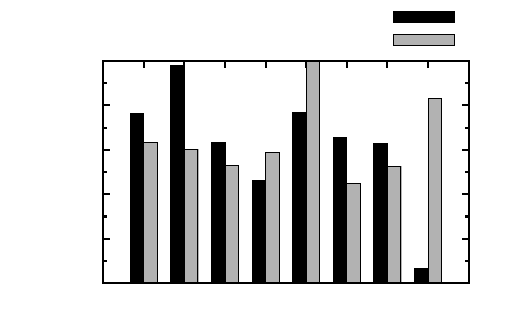
\includegraphics{plots/approxstats}}%
    \gplfronttext
  \end{picture}%
\endgroup

    \caption{
        Proportions of approximate writes and approximate data in
        each main-memory benchmark.
    }
    \label{approxstorage:fig:approxstats}
\end{figure}

Figure~\ref{approxstorage:fig:qos-mlc} relates write performance to application output
quality loss.
For configurations with fewer write iterations---to the
right-hand side of the plot---performance improves and quality declines. The
leftmost point in the plot is the nominal configuration, in which writes take
3.03 iterations on average and errors are rare. Reducing the number
of iterations has a direct impact on performance: a 50\% reduction in
iterations leads to 2$\times$ improvement in write speed.

The error for each application stays low for several configurations and then
increases sharply when hardware errors become too frequent.
The \textsf{raytracer} benchmark exhibits quality loss below 2\% up to the
configuration with 1.71 iterations per write on average, a $1.77\times$ speedup over the
baseline. Even the least tolerant application, \textsf{fft}, sees only
\result{fft-mlc-stripe-error}
quality loss when using an average of \result{fft-mlc-stripe-cycles} iterations per write (or
\result{fft-mlc-stripe-speedup} faster than the baseline).
This variance in tolerance suggests that
different applications have different optimal MLC configurations. Approximate
memories can accommodate these differences by exposing the threshold parameter $T$
for tuning.

To put these speedups in the context of the whole application, we
show the fraction of
dynamic writes that are to approximate data in
Figure~\ref{approxstorage:fig:approxstats}.
Most applications use approximate writes for
more than half of their stores; \textsf{jmeint} in particular has 98\%
approximate writes. One application, \textsf{zxing}, has a large amount of
``cold'' approximate data and benefits less from accelerating
approximate writes.


\paragraph{Persistent storage}

Figure~\ref{approxstorage:fig:nv-qos-mlc} shows the quality degradation for each
persistent data set when running on approximate MLC memory. The
persistent data sets we examine are more tolerant than the
main-memory benchmarks. The sensor logging application, for instance,
exhibits only \result{pa-mlc-stripe-error} quality degradation in the
configuration with \result{pa-mlc-stripe-cycles}
iterations per write (\result{pa-mlc-stripe-speedup} faster than the baseline) while the bitmap
image has only \result{image-mlc-stripe-error} quality degradation even in the most aggressive
configuration we examined, in which writes take
\result{image-mlc-stripe-cycles} cycles (\result{image-mlc-stripe-speedup}
faster than the baseline).
The neural network classifier, \textsf{ann}, experiences less than 10\%
recognition accuracy loss when using \result{nn-mlc-stripe-speedup} faster
writes; \textsf{svm}, in contrast, saw negligible accuracy loss in every
configuration we measured.

\vskip 12pt
\noindent
Overall, in the configurations with less than 10\% quality loss, the benchmarks
see \result{mlc-stripe-mean-speedup} faster writes to approximate cells over precise cells on
average.

This write latency reduction benefits application performance and memory
system power efficiency. Since write latency improvements reduce contention
and therefore also impact read latency, prior evaluations have found that they
can lead to large IPC increases~\cite{improvingwrites,powertokens}. Since fewer
programming pulses are used per write and write pulses make up a large portion
of PCM energy, the overall energy efficiency of the memory array is improved.

\paragraph{Impact of encoding}

Section~\ref{approxstorage:sec:coding} examines two different strategies for encoding
numeric values for storage on approximate MLCs. In the first, the bits from
multiple cells are concatenated to form whole words; in the second, each value
is ``striped'' across constituent cells so that the highest bits of the value
map to the highest bits of the cells. The results given above use
the latter encoding, but we also evaluated the simpler code for comparison.

The striped code leads to better output quality on average.
For three intermediate write speeds, using that code reduces the mean
output error across all applications from 1.1\% to 0.4\%, from 3.6\% to 3.0\%,
and from 11.0\% to 9.0\% with respect to the naive code.

We also
performed two-sample $t$-tests to assess the difference in output quality
between the two coding strategies for each of 13 write speed
configurations. For nearly every application, the striped code had a
statistically significant positive effect on quality more often than a
negative one. The only exception is \textsf{mc}, a Monte Carlo simulation, in
which the effect of the striped code was inconsistent (positive at some write
speeds and negative for others). 

While the striped code is imperfect, as
discussed in Section~\ref{approxstorage:sec:coding}, it fares better than the naive code in
practice since it lowers the probability of errors in the high-order bits of
words.


\paragraph{Density increase}

We experimented with adding more levels to an approximate MLC.
In a precise MLC, increasing
cell density requires more precise writes, but
approximate MLCs
can keep average write time
constant.
Our experiments show acceptable error rates when six levels are used (and no
other parameters are changed).
A non-power-of-two MLC requires additional hardware,
similar to binary-coded decimal (BCD) circuitry, to implement even the naive
code from Section~\ref{approxstorage:sec:coding} but can
still yield density benefits. For example, a 512-bit block can be stored in
$\lceil \frac{512}{\log 6} \rceil = 199$
six-level cells (compared to 256 four-level cells). With the same average number of
write iterations (3.03), many of our benchmarks
see little error: \textsf{jmeint}, \textsf{mc}, \textsf{raytracer},
\textsf{smm}, and the four persistent-storage benchmarks see error rates between
0.1\% and 4.2\%.
The other benchmarks, \textsf{fft}, \textsf{lu},
\textsf{sor}, and \textsf{zxing}, see high error rates, suggesting that
density increase should only be used with certain applications.

\paragraph{Impact of drift}

\begin{figure}
    \begin{subfigure}[b]{0.5\columnwidth}
        \centering
        % GNUPLOT: LaTeX picture with Postscript
\begingroup
\sffamily \footnotesize
  \makeatletter
  \providecommand\color[2][]{%
    \GenericError{(gnuplot) \space\space\space\@spaces}{%
      Package color not loaded in conjunction with
      terminal option `colourtext'%
    }{See the gnuplot documentation for explanation.%
    }{Either use 'blacktext' in gnuplot or load the package
      color.sty in LaTeX.}%
    \renewcommand\color[2][]{}%
  }%
  \providecommand\includegraphics[2][]{%
    \GenericError{(gnuplot) \space\space\space\@spaces}{%
      Package graphicx or graphics not loaded%
    }{See the gnuplot documentation for explanation.%
    }{The gnuplot epslatex terminal needs graphicx.sty or graphics.sty.}%
    \renewcommand\includegraphics[2][]{}%
  }%
  \providecommand\rotatebox[2]{#2}%
  \@ifundefined{ifGPcolor}{%
    \newif\ifGPcolor
    \GPcolorfalse
  }{}%
  \@ifundefined{ifGPblacktext}{%
    \newif\ifGPblacktext
    \GPblacktexttrue
  }{}%
  % define a \g@addto@macro without @ in the name:
  \let\gplgaddtomacro\g@addto@macro
  % define empty templates for all commands taking text:
  \gdef\gplbacktext{}%
  \gdef\gplfronttext{}%
  \makeatother
  \ifGPblacktext
    % no textcolor at all
    \def\colorrgb#1{}%
    \def\colorgray#1{}%
  \else
    % gray or color?
    \ifGPcolor
      \def\colorrgb#1{\color[rgb]{#1}}%
      \def\colorgray#1{\color[gray]{#1}}%
      \expandafter\def\csname LTw\endcsname{\color{white}}%
      \expandafter\def\csname LTb\endcsname{\color{black}}%
      \expandafter\def\csname LTa\endcsname{\color{black}}%
      \expandafter\def\csname LT0\endcsname{\color[rgb]{1,0,0}}%
      \expandafter\def\csname LT1\endcsname{\color[rgb]{0,1,0}}%
      \expandafter\def\csname LT2\endcsname{\color[rgb]{0,0,1}}%
      \expandafter\def\csname LT3\endcsname{\color[rgb]{1,0,1}}%
      \expandafter\def\csname LT4\endcsname{\color[rgb]{0,1,1}}%
      \expandafter\def\csname LT5\endcsname{\color[rgb]{1,1,0}}%
      \expandafter\def\csname LT6\endcsname{\color[rgb]{0,0,0}}%
      \expandafter\def\csname LT7\endcsname{\color[rgb]{1,0.3,0}}%
      \expandafter\def\csname LT8\endcsname{\color[rgb]{0.5,0.5,0.5}}%
    \else
      % gray
      \def\colorrgb#1{\color{black}}%
      \def\colorgray#1{\color[gray]{#1}}%
      \expandafter\def\csname LTw\endcsname{\color{white}}%
      \expandafter\def\csname LTb\endcsname{\color{black}}%
      \expandafter\def\csname LTa\endcsname{\color{black}}%
      \expandafter\def\csname LT0\endcsname{\color{black}}%
      \expandafter\def\csname LT1\endcsname{\color{black}}%
      \expandafter\def\csname LT2\endcsname{\color{black}}%
      \expandafter\def\csname LT3\endcsname{\color{black}}%
      \expandafter\def\csname LT4\endcsname{\color{black}}%
      \expandafter\def\csname LT5\endcsname{\color{black}}%
      \expandafter\def\csname LT6\endcsname{\color{black}}%
      \expandafter\def\csname LT7\endcsname{\color{black}}%
      \expandafter\def\csname LT8\endcsname{\color{black}}%
    \fi
  \fi
  \setlength{\unitlength}{0.0500bp}%
  \begin{picture}(4030.00,3628.00)%
    \gplgaddtomacro\gplbacktext{%
      \csname LTb\endcsname%
      \put(858,462){\makebox(0,0)[r]{\strut{}0\%}}%
      \put(858,886){\makebox(0,0)[r]{\strut{}20\%}}%
      \put(858,1310){\makebox(0,0)[r]{\strut{}40\%}}%
      \put(858,1734){\makebox(0,0)[r]{\strut{}60\%}}%
      \put(858,2158){\makebox(0,0)[r]{\strut{}80\%}}%
      \put(858,2582){\makebox(0,0)[r]{\strut{}100\%}}%
      \put(990,242){\makebox(0,0){\strut{}$10^1$}}%
      \put(1320,242){\makebox(0,0){\strut{}$10^2$}}%
      \put(1651,242){\makebox(0,0){\strut{}$10^3$}}%
      \put(1981,242){\makebox(0,0){\strut{}$10^4$}}%
      \put(2312,242){\makebox(0,0){\strut{}$10^5$}}%
      \put(2642,242){\makebox(0,0){\strut{}$10^6$}}%
      \put(2972,242){\makebox(0,0){\strut{}$10^7$}}%
      \put(3303,242){\makebox(0,0){\strut{}$10^8$}}%
      \put(3633,242){\makebox(0,0){\strut{}$10^9$}}%
      \put(286,1522){\rotatebox{-270}{\makebox(0,0){\strut{}output quality loss}}}%
      \put(2311,22){\makebox(0,0){\strut{}time (seconds)}}%
    }%
    \gplgaddtomacro\gplfronttext{%
      \csname LTb\endcsname%
      \put(1263,3455){\makebox(0,0)[r]{\strut{}fft}}%
      \csname LTb\endcsname%
      \put(1263,3235){\makebox(0,0)[r]{\strut{}zxing}}%
      \csname LTb\endcsname%
      \put(1263,3015){\makebox(0,0)[r]{\strut{}jmeint}}%
      \csname LTb\endcsname%
      \put(1263,2795){\makebox(0,0)[r]{\strut{}lu}}%
      \csname LTb\endcsname%
      \put(2778,3455){\makebox(0,0)[r]{\strut{}smm}}%
      \csname LTb\endcsname%
      \put(2778,3235){\makebox(0,0)[r]{\strut{}mc}}%
      \csname LTb\endcsname%
      \put(2778,3015){\makebox(0,0)[r]{\strut{}raytracer}}%
      \csname LTb\endcsname%
      \put(2778,2795){\makebox(0,0)[r]{\strut{}sor}}%
    }%
    \gplbacktext
    \put(0,0){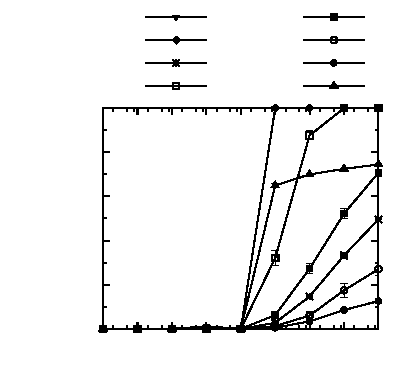
\includegraphics{plots/drift}}%
    \gplfronttext
  \end{picture}%
\endgroup

        \caption{
            Drift impact for main-memory applications.
        }
        \label{approxstorage:fig:mm-drift}
    \end{subfigure}
    \begin{subfigure}[b]{0.5\columnwidth}
        \centering
        % GNUPLOT: LaTeX picture with Postscript
\begingroup
\sffamily \footnotesize
  \makeatletter
  \providecommand\color[2][]{%
    \GenericError{(gnuplot) \space\space\space\@spaces}{%
      Package color not loaded in conjunction with
      terminal option `colourtext'%
    }{See the gnuplot documentation for explanation.%
    }{Either use 'blacktext' in gnuplot or load the package
      color.sty in LaTeX.}%
    \renewcommand\color[2][]{}%
  }%
  \providecommand\includegraphics[2][]{%
    \GenericError{(gnuplot) \space\space\space\@spaces}{%
      Package graphicx or graphics not loaded%
    }{See the gnuplot documentation for explanation.%
    }{The gnuplot epslatex terminal needs graphicx.sty or graphics.sty.}%
    \renewcommand\includegraphics[2][]{}%
  }%
  \providecommand\rotatebox[2]{#2}%
  \@ifundefined{ifGPcolor}{%
    \newif\ifGPcolor
    \GPcolorfalse
  }{}%
  \@ifundefined{ifGPblacktext}{%
    \newif\ifGPblacktext
    \GPblacktexttrue
  }{}%
  % define a \g@addto@macro without @ in the name:
  \let\gplgaddtomacro\g@addto@macro
  % define empty templates for all commands taking text:
  \gdef\gplbacktext{}%
  \gdef\gplfronttext{}%
  \makeatother
  \ifGPblacktext
    % no textcolor at all
    \def\colorrgb#1{}%
    \def\colorgray#1{}%
  \else
    % gray or color?
    \ifGPcolor
      \def\colorrgb#1{\color[rgb]{#1}}%
      \def\colorgray#1{\color[gray]{#1}}%
      \expandafter\def\csname LTw\endcsname{\color{white}}%
      \expandafter\def\csname LTb\endcsname{\color{black}}%
      \expandafter\def\csname LTa\endcsname{\color{black}}%
      \expandafter\def\csname LT0\endcsname{\color[rgb]{1,0,0}}%
      \expandafter\def\csname LT1\endcsname{\color[rgb]{0,1,0}}%
      \expandafter\def\csname LT2\endcsname{\color[rgb]{0,0,1}}%
      \expandafter\def\csname LT3\endcsname{\color[rgb]{1,0,1}}%
      \expandafter\def\csname LT4\endcsname{\color[rgb]{0,1,1}}%
      \expandafter\def\csname LT5\endcsname{\color[rgb]{1,1,0}}%
      \expandafter\def\csname LT6\endcsname{\color[rgb]{0,0,0}}%
      \expandafter\def\csname LT7\endcsname{\color[rgb]{1,0.3,0}}%
      \expandafter\def\csname LT8\endcsname{\color[rgb]{0.5,0.5,0.5}}%
    \else
      % gray
      \def\colorrgb#1{\color{black}}%
      \def\colorgray#1{\color[gray]{#1}}%
      \expandafter\def\csname LTw\endcsname{\color{white}}%
      \expandafter\def\csname LTb\endcsname{\color{black}}%
      \expandafter\def\csname LTa\endcsname{\color{black}}%
      \expandafter\def\csname LT0\endcsname{\color{black}}%
      \expandafter\def\csname LT1\endcsname{\color{black}}%
      \expandafter\def\csname LT2\endcsname{\color{black}}%
      \expandafter\def\csname LT3\endcsname{\color{black}}%
      \expandafter\def\csname LT4\endcsname{\color{black}}%
      \expandafter\def\csname LT5\endcsname{\color{black}}%
      \expandafter\def\csname LT6\endcsname{\color{black}}%
      \expandafter\def\csname LT7\endcsname{\color{black}}%
      \expandafter\def\csname LT8\endcsname{\color{black}}%
    \fi
  \fi
  \setlength{\unitlength}{0.0500bp}%
  \begin{picture}(4030.00,3168.00)%
    \gplgaddtomacro\gplbacktext{%
      \csname LTb\endcsname%
      \put(858,462){\makebox(0,0)[r]{\strut{}0\%}}%
      \put(858,884){\makebox(0,0)[r]{\strut{}20\%}}%
      \put(858,1306){\makebox(0,0)[r]{\strut{}40\%}}%
      \put(858,1729){\makebox(0,0)[r]{\strut{}60\%}}%
      \put(858,2151){\makebox(0,0)[r]{\strut{}80\%}}%
      \put(858,2573){\makebox(0,0)[r]{\strut{}100\%}}%
      \put(990,242){\makebox(0,0){\strut{}$10^1$}}%
      \put(1320,242){\makebox(0,0){\strut{}$10^2$}}%
      \put(1651,242){\makebox(0,0){\strut{}$10^3$}}%
      \put(1981,242){\makebox(0,0){\strut{}$10^4$}}%
      \put(2312,242){\makebox(0,0){\strut{}$10^5$}}%
      \put(2642,242){\makebox(0,0){\strut{}$10^6$}}%
      \put(2972,242){\makebox(0,0){\strut{}$10^7$}}%
      \put(3303,242){\makebox(0,0){\strut{}$10^8$}}%
      \put(3633,242){\makebox(0,0){\strut{}$10^9$}}%
      \put(286,1517){\rotatebox{-270}{\makebox(0,0){\strut{}output quality loss}}}%
      \put(2311,22){\makebox(0,0){\strut{}time (seconds)}}%
    }%
    \gplgaddtomacro\gplfronttext{%
      \csname LTb\endcsname%
      \put(1263,2995){\makebox(0,0)[r]{\strut{}ann}}%
      \csname LTb\endcsname%
      \put(1263,2775){\makebox(0,0)[r]{\strut{}sensorlog}}%
      \csname LTb\endcsname%
      \put(2778,2995){\makebox(0,0)[r]{\strut{}image}}%
      \csname LTb\endcsname%
      \put(2778,2775){\makebox(0,0)[r]{\strut{}svm}}%
    }%
    \gplbacktext
    \put(0,0){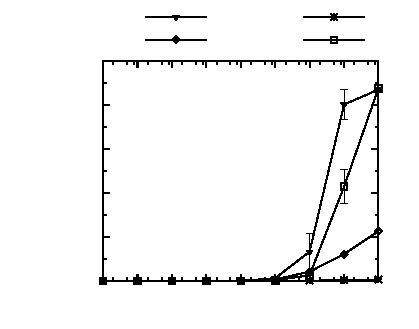
\includegraphics{plots/nv_drift}}%
    \gplfronttext
  \end{picture}%
\endgroup

        \caption{
            Drift impact for persistent data sets.
        }
        \label{approxstorage:fig:nv-drift}
    \end{subfigure}
    \caption{
        Application output quality over time using the approximate MLC
        technique using 2.1 cycles per write.
        Drift causes errors to increase in proportion to the time
        since the last write to the PCM cell.
    }
    \label{approxstorage:fig:drift}
\end{figure}

Previous work has suggested that straightforward MLC storage in PCM can be
untenable over long periods of time~\cite{wdddmlcpcm}.
Approximate storage provides an opportunity to reduce the frequency of
scrubbing necessary by tolerating occasional retention errors.
To study the resilience of approximate MLC storage to drift,
we varied the modeled retention time (the interval between write and read) and
examined the resulting application-level quality loss.
Recall that the results
above assume a retention time of $10^5$ seconds, or about one day, for every
read operation; we examined retention times between $10^1$ and $10^9$ seconds
(about 80 years) for an intermediate approximate MLC configuration using an
average of 2.1 cycles per write.

Figure~\ref{approxstorage:fig:drift} depicts the application output quality for a range of
time intervals.
For the main-memory applications in Figure~\ref{approxstorage:fig:mm-drift}, in which typical retention times are
likely far less than one day, we see little quality loss (1\% or
less) for retention times of $10^4$ seconds or shorter.
As above, these simulations assume the same drift interval for \emph{every}
read.
In this sense, the results are pessimistic since many reads
are to recently written data and therefore incur less error from
drift.

For the
persistent-storage benchmarks in Figure~\ref{approxstorage:fig:nv-drift}, in contrast, longer retention times are the
norm.
In that setting, quality loss remains under 10\% for at least
$10^6$ seconds and, for all benchmarks except \textsf{ann}, through $10^7$ seconds.
The most tolerant data set, \textsf{image}, remains below 10\% error for
$10^9$ seconds of drift.
The persistent-storage benchmarks tend to be more resilient to drift because
the stored data tends to be uniformly error tolerant: every neuron weight or
every pixel contributes equally to the quality of the output.
This uniformity contrasts with the main-memory applications, where certain
``hot'' data structures are more critical for quality and therefore
tolerate less error.

A longer retention time means scrubbing can be done less frequently.
The above results report the quality impact of one retention cycle:
the persistent-storage benchmarks, for example, lose less than 10\%
of their quality when $10^6$ seconds, or about 11 days, elapse after they are
first written to memory assuming no scrubbing occurs in that time.
Eleven more days of drift will compound additional error.
While the results suggest that the more error-tolerant applications can
tolerate longer scrubbing cycles, we do not measure how error compounds over
longer-term storage periods with infrequent scrubbing.

\paragraph{Bit error rate}

To add context to the output quality results above, we also measured the
effective bit error rate (BER) of approximate MLC storage. The BER is the
probability that a bit read from approximate memory is different from
the corresponding last bit written.
Across the write speeds we examined, error rates range from $3.7
\times 10^{-7}$ to $8.4\%$ in the most aggressive configuration.
%
To put these rates in perspective, if the bit error rate is $p$, then a 64-bit
block will have at least 2 errors with probability $\sum_{i = 2}^{64} B(i, 64,
p)$ where $B$ is the binomial distribution. At a moderately aggressive write
speed configuration with an average of 1.9 steps, approximate MLC storage has
an error rate of $7.2 \times 10^{-4}$, so 0.1\% of 64-bit
words have 2 or more errors. This high error rate demonstrates the need
for application-level error tolerance: even strong ECC with two-bit correction
will not suffice to provide precise storage under such frequent errors.


\subsection{Using Failed Blocks}

We evaluate the failed-block recycling technique by simulating
benchmarks on PCM arrays in varying stages of wear-out. As the
memory device ages and cells fail, some blocks exhaust their
error-correction budget. Approximate data is then mapped onto these
blocks.
Over the array's lifetime,
bit errors in approximate memory
become more common. Eventually, these errors impact the application to such a
degree that the computation quality is no longer acceptable, at which point the
memory array must be replaced.
We quantify the
lifetime extension afforded by this technique, beginning with the
main-memory applications.

To quantify lifetime extension, we assume a memory module with a 10\% ``space
margin'': 10\% of the memory is reserved to allow for some block
failures before the array must be replaced. In the baseline precise
configuration, the array fails when the fraction of blocks that remain
precise (having only correctable failures) drops below 90\%. In the approximate
configuration, programs continue to run until there is not enough space for
their precise data or quality drops below a threshold.

\paragraph{Approximate main memory}

\begin{figure}
    \centering
    % GNUPLOT: LaTeX picture with Postscript
\begingroup
\sffamily \footnotesize
  \makeatletter
  \providecommand\color[2][]{%
    \GenericError{(gnuplot) \space\space\space\@spaces}{%
      Package color not loaded in conjunction with
      terminal option `colourtext'%
    }{See the gnuplot documentation for explanation.%
    }{Either use 'blacktext' in gnuplot or load the package
      color.sty in LaTeX.}%
    \renewcommand\color[2][]{}%
  }%
  \providecommand\includegraphics[2][]{%
    \GenericError{(gnuplot) \space\space\space\@spaces}{%
      Package graphicx or graphics not loaded%
    }{See the gnuplot documentation for explanation.%
    }{The gnuplot epslatex terminal needs graphicx.sty or graphics.sty.}%
    \renewcommand\includegraphics[2][]{}%
  }%
  \providecommand\rotatebox[2]{#2}%
  \@ifundefined{ifGPcolor}{%
    \newif\ifGPcolor
    \GPcolorfalse
  }{}%
  \@ifundefined{ifGPblacktext}{%
    \newif\ifGPblacktext
    \GPblacktexttrue
  }{}%
  % define a \g@addto@macro without @ in the name:
  \let\gplgaddtomacro\g@addto@macro
  % define empty templates for all commands taking text:
  \gdef\gplbacktext{}%
  \gdef\gplfronttext{}%
  \makeatother
  \ifGPblacktext
    % no textcolor at all
    \def\colorrgb#1{}%
    \def\colorgray#1{}%
  \else
    % gray or color?
    \ifGPcolor
      \def\colorrgb#1{\color[rgb]{#1}}%
      \def\colorgray#1{\color[gray]{#1}}%
      \expandafter\def\csname LTw\endcsname{\color{white}}%
      \expandafter\def\csname LTb\endcsname{\color{black}}%
      \expandafter\def\csname LTa\endcsname{\color{black}}%
      \expandafter\def\csname LT0\endcsname{\color[rgb]{1,0,0}}%
      \expandafter\def\csname LT1\endcsname{\color[rgb]{0,1,0}}%
      \expandafter\def\csname LT2\endcsname{\color[rgb]{0,0,1}}%
      \expandafter\def\csname LT3\endcsname{\color[rgb]{1,0,1}}%
      \expandafter\def\csname LT4\endcsname{\color[rgb]{0,1,1}}%
      \expandafter\def\csname LT5\endcsname{\color[rgb]{1,1,0}}%
      \expandafter\def\csname LT6\endcsname{\color[rgb]{0,0,0}}%
      \expandafter\def\csname LT7\endcsname{\color[rgb]{1,0.3,0}}%
      \expandafter\def\csname LT8\endcsname{\color[rgb]{0.5,0.5,0.5}}%
    \else
      % gray
      \def\colorrgb#1{\color{black}}%
      \def\colorgray#1{\color[gray]{#1}}%
      \expandafter\def\csname LTw\endcsname{\color{white}}%
      \expandafter\def\csname LTb\endcsname{\color{black}}%
      \expandafter\def\csname LTa\endcsname{\color{black}}%
      \expandafter\def\csname LT0\endcsname{\color{black}}%
      \expandafter\def\csname LT1\endcsname{\color{black}}%
      \expandafter\def\csname LT2\endcsname{\color{black}}%
      \expandafter\def\csname LT3\endcsname{\color{black}}%
      \expandafter\def\csname LT4\endcsname{\color{black}}%
      \expandafter\def\csname LT5\endcsname{\color{black}}%
      \expandafter\def\csname LT6\endcsname{\color{black}}%
      \expandafter\def\csname LT7\endcsname{\color{black}}%
      \expandafter\def\csname LT8\endcsname{\color{black}}%
    \fi
  \fi
  \setlength{\unitlength}{0.0500bp}%
  \begin{picture}(4896.00,2880.00)%
    \gplgaddtomacro\gplbacktext{%
      \csname LTb\endcsname%
      \put(594,440){\makebox(0,0)[r]{\strut{}0.0}}%
      \put(594,704){\makebox(0,0)[r]{\strut{}0.2}}%
      \put(594,967){\makebox(0,0)[r]{\strut{}0.4}}%
      \put(594,1231){\makebox(0,0)[r]{\strut{}0.6}}%
      \put(594,1494){\makebox(0,0)[r]{\strut{}0.8}}%
      \put(594,1758){\makebox(0,0)[r]{\strut{}1.0}}%
      \put(594,2021){\makebox(0,0)[r]{\strut{}1.2}}%
      \put(594,2285){\makebox(0,0)[r]{\strut{}1.4}}%
      \put(1145,220){\makebox(0,0){\strut{}fft}}%
      \put(1564,220){\makebox(0,0){\strut{}jmeint}}%
      \put(1984,220){\makebox(0,0){\strut{}lu}}%
      \put(2403,220){\makebox(0,0){\strut{}mc}}%
      \put(2822,220){\makebox(0,0){\strut{}raytr.}}%
      \put(3241,220){\makebox(0,0){\strut{}smm}}%
      \put(3661,220){\makebox(0,0){\strut{}sor}}%
      \put(4080,220){\makebox(0,0){\strut{}zxing}}%
      \put(233,1362){\rotatebox{-270}{\makebox(0,0){\strut{}normalized lifetime (writes)}}}%
    }%
    \gplgaddtomacro\gplfronttext{%
      \csname LTb\endcsname%
      \put(3644,2707){\makebox(0,0)[r]{\strut{}insufficient precise blocks}}%
      \csname LTb\endcsname%
      \put(3644,2487){\makebox(0,0)[r]{\strut{}quality loss exceeds 10\%}}%
    }%
    \gplbacktext
    \put(0,0){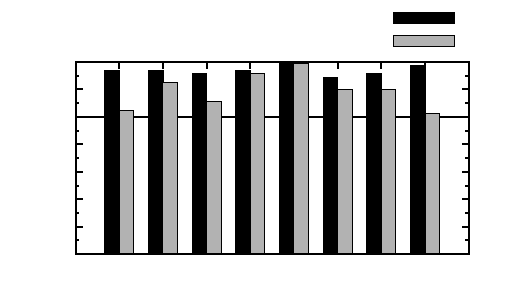
\includegraphics{plots/extension_persistent-tbec2}}%
    \gplfronttext
  \end{picture}%
\endgroup

    \caption{
        Lifetime extension for each application.
    Each bar represents the number of writes to the entire array at
    which the application can no longer run,
    normalized to the point of array failure in fully-precise mode.
    The black bar indicates when there is not enough precise
    memory available. The gray bar shows when the application's
    output quality degrades more than 10\%.
    }
    \label{approxstorage:fig:extension}
\end{figure}

\begin{figure}
    \begin{subfigure}[b]{0.5\columnwidth}
        \centering
        % GNUPLOT: LaTeX picture with Postscript
\begingroup
\sffamily \footnotesize
  \makeatletter
  \providecommand\color[2][]{%
    \GenericError{(gnuplot) \space\space\space\@spaces}{%
      Package color not loaded in conjunction with
      terminal option `colourtext'%
    }{See the gnuplot documentation for explanation.%
    }{Either use 'blacktext' in gnuplot or load the package
      color.sty in LaTeX.}%
    \renewcommand\color[2][]{}%
  }%
  \providecommand\includegraphics[2][]{%
    \GenericError{(gnuplot) \space\space\space\@spaces}{%
      Package graphicx or graphics not loaded%
    }{See the gnuplot documentation for explanation.%
    }{The gnuplot epslatex terminal needs graphicx.sty or graphics.sty.}%
    \renewcommand\includegraphics[2][]{}%
  }%
  \providecommand\rotatebox[2]{#2}%
  \@ifundefined{ifGPcolor}{%
    \newif\ifGPcolor
    \GPcolorfalse
  }{}%
  \@ifundefined{ifGPblacktext}{%
    \newif\ifGPblacktext
    \GPblacktexttrue
  }{}%
  % define a \g@addto@macro without @ in the name:
  \let\gplgaddtomacro\g@addto@macro
  % define empty templates for all commands taking text:
  \gdef\gplbacktext{}%
  \gdef\gplfronttext{}%
  \makeatother
  \ifGPblacktext
    % no textcolor at all
    \def\colorrgb#1{}%
    \def\colorgray#1{}%
  \else
    % gray or color?
    \ifGPcolor
      \def\colorrgb#1{\color[rgb]{#1}}%
      \def\colorgray#1{\color[gray]{#1}}%
      \expandafter\def\csname LTw\endcsname{\color{white}}%
      \expandafter\def\csname LTb\endcsname{\color{black}}%
      \expandafter\def\csname LTa\endcsname{\color{black}}%
      \expandafter\def\csname LT0\endcsname{\color[rgb]{1,0,0}}%
      \expandafter\def\csname LT1\endcsname{\color[rgb]{0,1,0}}%
      \expandafter\def\csname LT2\endcsname{\color[rgb]{0,0,1}}%
      \expandafter\def\csname LT3\endcsname{\color[rgb]{1,0,1}}%
      \expandafter\def\csname LT4\endcsname{\color[rgb]{0,1,1}}%
      \expandafter\def\csname LT5\endcsname{\color[rgb]{1,1,0}}%
      \expandafter\def\csname LT6\endcsname{\color[rgb]{0,0,0}}%
      \expandafter\def\csname LT7\endcsname{\color[rgb]{1,0.3,0}}%
      \expandafter\def\csname LT8\endcsname{\color[rgb]{0.5,0.5,0.5}}%
    \else
      % gray
      \def\colorrgb#1{\color{black}}%
      \def\colorgray#1{\color[gray]{#1}}%
      \expandafter\def\csname LTw\endcsname{\color{white}}%
      \expandafter\def\csname LTb\endcsname{\color{black}}%
      \expandafter\def\csname LTa\endcsname{\color{black}}%
      \expandafter\def\csname LT0\endcsname{\color{black}}%
      \expandafter\def\csname LT1\endcsname{\color{black}}%
      \expandafter\def\csname LT2\endcsname{\color{black}}%
      \expandafter\def\csname LT3\endcsname{\color{black}}%
      \expandafter\def\csname LT4\endcsname{\color{black}}%
      \expandafter\def\csname LT5\endcsname{\color{black}}%
      \expandafter\def\csname LT6\endcsname{\color{black}}%
      \expandafter\def\csname LT7\endcsname{\color{black}}%
      \expandafter\def\csname LT8\endcsname{\color{black}}%
    \fi
  \fi
  \setlength{\unitlength}{0.0500bp}%
  \begin{picture}(4030.00,3628.00)%
    \gplgaddtomacro\gplbacktext{%
      \csname LTb\endcsname%
      \put(858,462){\makebox(0,0)[r]{\strut{}0\%}}%
      \put(858,886){\makebox(0,0)[r]{\strut{}20\%}}%
      \put(858,1310){\makebox(0,0)[r]{\strut{}40\%}}%
      \put(858,1734){\makebox(0,0)[r]{\strut{}60\%}}%
      \put(858,2158){\makebox(0,0)[r]{\strut{}80\%}}%
      \put(858,2582){\makebox(0,0)[r]{\strut{}100\%}}%
      \put(1222,242){\makebox(0,0){\strut{} 2.2}}%
      \put(1620,242){\makebox(0,0){\strut{} 2.4}}%
      \put(2019,242){\makebox(0,0){\strut{} 2.6}}%
      \put(2417,242){\makebox(0,0){\strut{} 2.8}}%
      \put(2816,242){\makebox(0,0){\strut{} 3}}%
      \put(3214,242){\makebox(0,0){\strut{} 3.2}}%
      \put(3613,242){\makebox(0,0){\strut{} 3.4}}%
      \put(286,1522){\rotatebox{-270}{\makebox(0,0){\strut{}output quality loss}}}%
      \put(2311,22){\makebox(0,0){\strut{}writes $\times 10^{7}$}}%
    }%
    \gplgaddtomacro\gplfronttext{%
      \csname LTb\endcsname%
      \put(1263,3455){\makebox(0,0)[r]{\strut{}fft}}%
      \csname LTb\endcsname%
      \put(1263,3235){\makebox(0,0)[r]{\strut{}zxing}}%
      \csname LTb\endcsname%
      \put(1263,3015){\makebox(0,0)[r]{\strut{}jmeint}}%
      \csname LTb\endcsname%
      \put(1263,2795){\makebox(0,0)[r]{\strut{}lu}}%
      \csname LTb\endcsname%
      \put(2778,3455){\makebox(0,0)[r]{\strut{}smm}}%
      \csname LTb\endcsname%
      \put(2778,3235){\makebox(0,0)[r]{\strut{}mc}}%
      \csname LTb\endcsname%
      \put(2778,3015){\makebox(0,0)[r]{\strut{}raytracer}}%
      \csname LTb\endcsname%
      \put(2778,2795){\makebox(0,0)[r]{\strut{}sor}}%
    }%
    \gplbacktext
    \put(0,0){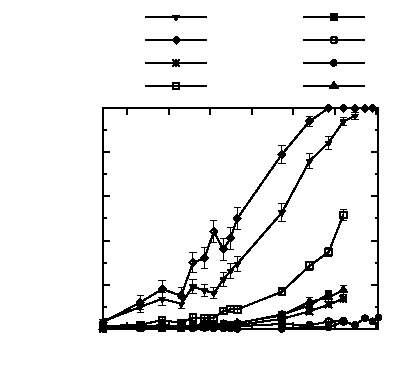
\includegraphics{plots/qos_persistent-tbec2}}%
    \gplfronttext
  \end{picture}%
\endgroup

        \caption{
            Main-memory applications using failed blocks.
        }
        \label{approxstorage:fig:qos-p-tb}
    \end{subfigure}
    \begin{subfigure}[b]{0.5\columnwidth}
        \centering
        % GNUPLOT: LaTeX picture with Postscript
\begingroup
\sffamily \footnotesize
  \makeatletter
  \providecommand\color[2][]{%
    \GenericError{(gnuplot) \space\space\space\@spaces}{%
      Package color not loaded in conjunction with
      terminal option `colourtext'%
    }{See the gnuplot documentation for explanation.%
    }{Either use 'blacktext' in gnuplot or load the package
      color.sty in LaTeX.}%
    \renewcommand\color[2][]{}%
  }%
  \providecommand\includegraphics[2][]{%
    \GenericError{(gnuplot) \space\space\space\@spaces}{%
      Package graphicx or graphics not loaded%
    }{See the gnuplot documentation for explanation.%
    }{The gnuplot epslatex terminal needs graphicx.sty or graphics.sty.}%
    \renewcommand\includegraphics[2][]{}%
  }%
  \providecommand\rotatebox[2]{#2}%
  \@ifundefined{ifGPcolor}{%
    \newif\ifGPcolor
    \GPcolorfalse
  }{}%
  \@ifundefined{ifGPblacktext}{%
    \newif\ifGPblacktext
    \GPblacktexttrue
  }{}%
  % define a \g@addto@macro without @ in the name:
  \let\gplgaddtomacro\g@addto@macro
  % define empty templates for all commands taking text:
  \gdef\gplbacktext{}%
  \gdef\gplfronttext{}%
  \makeatother
  \ifGPblacktext
    % no textcolor at all
    \def\colorrgb#1{}%
    \def\colorgray#1{}%
  \else
    % gray or color?
    \ifGPcolor
      \def\colorrgb#1{\color[rgb]{#1}}%
      \def\colorgray#1{\color[gray]{#1}}%
      \expandafter\def\csname LTw\endcsname{\color{white}}%
      \expandafter\def\csname LTb\endcsname{\color{black}}%
      \expandafter\def\csname LTa\endcsname{\color{black}}%
      \expandafter\def\csname LT0\endcsname{\color[rgb]{1,0,0}}%
      \expandafter\def\csname LT1\endcsname{\color[rgb]{0,1,0}}%
      \expandafter\def\csname LT2\endcsname{\color[rgb]{0,0,1}}%
      \expandafter\def\csname LT3\endcsname{\color[rgb]{1,0,1}}%
      \expandafter\def\csname LT4\endcsname{\color[rgb]{0,1,1}}%
      \expandafter\def\csname LT5\endcsname{\color[rgb]{1,1,0}}%
      \expandafter\def\csname LT6\endcsname{\color[rgb]{0,0,0}}%
      \expandafter\def\csname LT7\endcsname{\color[rgb]{1,0.3,0}}%
      \expandafter\def\csname LT8\endcsname{\color[rgb]{0.5,0.5,0.5}}%
    \else
      % gray
      \def\colorrgb#1{\color{black}}%
      \def\colorgray#1{\color[gray]{#1}}%
      \expandafter\def\csname LTw\endcsname{\color{white}}%
      \expandafter\def\csname LTb\endcsname{\color{black}}%
      \expandafter\def\csname LTa\endcsname{\color{black}}%
      \expandafter\def\csname LT0\endcsname{\color{black}}%
      \expandafter\def\csname LT1\endcsname{\color{black}}%
      \expandafter\def\csname LT2\endcsname{\color{black}}%
      \expandafter\def\csname LT3\endcsname{\color{black}}%
      \expandafter\def\csname LT4\endcsname{\color{black}}%
      \expandafter\def\csname LT5\endcsname{\color{black}}%
      \expandafter\def\csname LT6\endcsname{\color{black}}%
      \expandafter\def\csname LT7\endcsname{\color{black}}%
      \expandafter\def\csname LT8\endcsname{\color{black}}%
    \fi
  \fi
  \setlength{\unitlength}{0.0500bp}%
  \begin{picture}(4030.00,3168.00)%
    \gplgaddtomacro\gplbacktext{%
      \csname LTb\endcsname%
      \put(858,462){\makebox(0,0)[r]{\strut{}0\%}}%
      \put(858,884){\makebox(0,0)[r]{\strut{}20\%}}%
      \put(858,1306){\makebox(0,0)[r]{\strut{}40\%}}%
      \put(858,1729){\makebox(0,0)[r]{\strut{}60\%}}%
      \put(858,2151){\makebox(0,0)[r]{\strut{}80\%}}%
      \put(858,2573){\makebox(0,0)[r]{\strut{}100\%}}%
      \put(1345,242){\makebox(0,0){\strut{} 4}}%
      \put(1756,242){\makebox(0,0){\strut{} 4.5}}%
      \put(2168,242){\makebox(0,0){\strut{} 5}}%
      \put(2579,242){\makebox(0,0){\strut{} 5.5}}%
      \put(2990,242){\makebox(0,0){\strut{} 6}}%
      \put(3401,242){\makebox(0,0){\strut{} 6.5}}%
      \put(286,1517){\rotatebox{-270}{\makebox(0,0){\strut{}output quality loss}}}%
      \put(2311,22){\makebox(0,0){\strut{}writes $\times 10^{7}$}}%
    }%
    \gplgaddtomacro\gplfronttext{%
      \csname LTb\endcsname%
      \put(1263,2995){\makebox(0,0)[r]{\strut{}ann}}%
      \csname LTb\endcsname%
      \put(1263,2775){\makebox(0,0)[r]{\strut{}sensorlog}}%
      \csname LTb\endcsname%
      \put(2778,2995){\makebox(0,0)[r]{\strut{}image}}%
      \csname LTb\endcsname%
      \put(2778,2775){\makebox(0,0)[r]{\strut{}svm}}%
    }%
    \gplbacktext
    \put(0,0){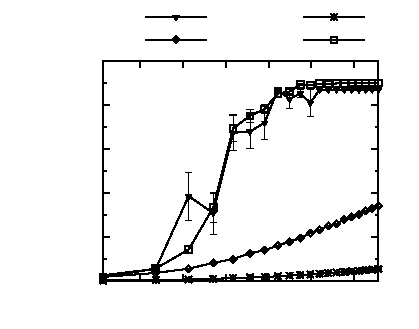
\includegraphics{plots/nv_qos_a-tbec2}}%
    \gplfronttext
  \end{picture}%
\endgroup

        \caption{
            Persistent data sets using failed blocks.
        }
        \label{approxstorage:fig:nv-qos-tb}
    \end{subfigure}
    \caption{
        Output quality degradation for each benchmark when using the
        failed-block recycling technique. The horizontal axis is the number of
        complete overwrites the array has experienced, indicating the stage of
        wear-out. The vertical axis is an application-specific error metric.
    }
\end{figure}

Figure~\ref{approxstorage:fig:extension} depicts the lifetime extension afforded by
using failed blocks as approximate storage. For
each application, we determine the point in the memory's lifetime
(under the wear model described in Section~\ref{approxstorage:sec:wearmodel}) at
which the program can no longer run. We consider two termination
conditions: when the amount of
precise memory becomes insufficient (i.e., the proportion of
approximate memory exceeds the application's proportion of approximate
data) and when the application's output quality degrades more than 10\%. Each bar in
the figure shows the normalized number of writes to the memory when
application failure occurs.

With quality degradation limited to 10\%, the benchmarks see lifetime
extensions ranging from \result{recycle-zxing-qos-ext} (\textsf{zxing}) to
\result{recycle-raytracer-qos-ext} (\textsf{raytracer}) with
a harmonic mean of \result{recycle-mean-qos-ext}. With quality unconstrained, the mean lifetime
extension is \result{recycle-mean-total-ext}, reflecting the fact that this technique leads to gradually
decreasing quality as the memory array ages.

To help explain these results, Figure~\ref{approxstorage:fig:qos-p-tb} shows the quality
degradation for each application at various points during the memory array's
wear-out.
The most error-tolerant application, \textsf{raytracer}, sees
little quality degradation under all measured wear stages.
Some applications are limited by the amount of approximate data they use.
Figure~\ref{approxstorage:fig:approxstats} shows the proportion of bytes in each
application's memory that is approximate (averaged over the execution).
Some applications,
such as \textsf{mc}, are tolerant to error but only have around 50\%
approximate data. In other
cases, such as \textsf{zxing} and \textsf{fft}, bit errors
have a large effect on the computation quality. In \textsf{fft} in
particular, we find that a single floating-point intermediate value that
becomes \verb+NaN+ can contaminate the Fourier transform's entire output.
This suggests that the application's precision
annotations, which determine which data is stored approximately, may be
too aggressive.

\paragraph{Persistent storage}

Figure~\ref{approxstorage:fig:nv-qos-tb} shows the quality degradation for each data set at
different points during the lifetime of the memory.
The memory's intermediate
wear-out conditions come from the persistent-storage wear model described in
Section~\ref{approxstorage:sec:wearmodel}.
In a fully-precise configuration, the memory fails (exceeds 10\% failed blocks)
at about $3.4 \times 10^{7}$ overwrites, or at the left-hand side of the plot.
Recall that, in these persistent-storage benchmarks, the data is stored 100\%
approximately; no precise storage is used.

As with the main-memory storage setting, quality decreases over time as errors
become more frequent. But these benchmarks are more tolerant to stuck bits
than the main-memory applications. For \textsf{image}, quality loss is below
10\% in all wear stages; for \textsf{sensorlog}, it remains below 10\% until
the array experiences
$5.0 \times 10^{7}$ writes, or \result{recycle-pa-ext} later than precise array failure.
The two machine learning classifiers, \textsf{ann} and \textsf{svm},
each see lifetime extensions of 17\%.
This tolerance to
stuck bits makes the failed-block recycling technique particularly attractive
for persistent storage scenarios with large amounts of numeric data.

\vskip 12pt
\noindent
Overall, across both categories of benchmarks, we see a harmonic mean
lifetime extension of \result{recycle-mean-all-ext}
(\result{recycle-mean-qos-ext} for the main-memory benchmarks and
\result{recycle-mean-nv-ext} for
the persistent-storage data sets) when quality loss is limited to 10\%.
Recent work has demonstrated PCM arrays that sustain a random write bandwidth of
1.5~GB/s~\cite{moneta};
for a 10~GB memory constantly written at this rate,
these savings translate to extending the array's lifetime
from 5.2 years to 6.5 years.

\paragraph{Impact of bit priority} The above results use our type-aware
prioritized correction mechanism (Section~\ref{approxstorage:sec:bitprior}). To evaluate the
impact of bit prioritization, we ran a separate set of experiments with this
mechanism disabled to model a system that just corrects the errors that
occur earliest. We examine the difference in output quality at each wear stage and
perform a two-sample $t$-test to determine whether the difference is
statistically significant ($P < 0.01$).

Bit prioritization had a statistically significant positive impact on output
quality for all benchmarks except \textsf{mc}. In \textsf{sensorlog}, for example, bit
prioritization decreases quality loss from 2.3\% to 1.7\% in an early stage of
wear (the leftmost point in Figure~\ref{approxstorage:fig:nv-qos-tb}). In \textsf{fft}, the
impact is larger: bit prioritization reduces 7.3\% quality loss to
3.3\% quality loss. As with encoding for approximate MLCs, the exception is \textsf{mc}, whose quality was
(statistically significantly) improved in
only 4 of the 45 wear stages we measured while it was \emph{negatively}
impacted in 6 wear stages. This benchmark is a simple Monte Carlo method
and hence may sometimes \emph{benefit} from the entropy added by failed bits.
Overall, however, we conclude that bit prioritization has a generally positive
effect on storage quality.

\paragraph{Impact of ECP budget} The above experiments use a PCM configuration
with error-correcting pointers (ECP)~\cite{ecp} configured to correct two stuck
bits per 512-bit block at an overhead of 21 extra bits per block. More
aggressive error correction improves the endurance of both fully-precise and
approximate memory and amplifies the opportunity for priority-aware
correction in intermediate wear stages. To quantify the effect of increasing
error correction budgets, we also evaluated an ECP$_6$ configuration (61 extra
bits per block).

Moving from ECP$_2$ to ECP$_6$ extends the lifetime of a precise memory array
by 45\% under main-memory wear or 17\% under persistent-storage wear.
Our
results for approximate main-memory storage with ECP$_2$ provide a
portion of these benefits (\result{recycle-mean-qos-ext} lifetime extension) while incurring no
additional error-correction overhead. In the persistent-storage case, the
lifetime extension for approximate storage (\result{recycle-mean-nv-ext}) is greater than for
increasing the ECP budget.

% Relative to a precise ECP$_6$ baseline, approximate ECP$_6$ offers an average
% lifetime extension of 11\% for the main-memory benchmarks, 42\% for
% the persistent-storage data sets, or 16\% overall with quality loss limited
% to 10\%.

% 2->6 extension for NV: 17% (2.99 -> 3.50 x 10^14 writes)
% for MM: 45% (2.06 -> 3.00)


\section{Related Work}
\label{approxstorage:sec:related}

Approximate storage builds on three broad categories of related work:
approximate computing, optimizing accesses to storage
cells, and tolerating failures in solid-state memories.

Approximate computing is an area of research that seeks to optimize the
execution of error-tolerant programs using both
hardware~\cite{flikker,truffle,npu,relax,pcmos,stochasticproc} and software~\cite{green,perforation,dynamicknobs} techniques. Programmers control the impact of approximate execution using language features, analyses, or program
logics~\cite{enerj,relax,carbin_pldi12,rely}. While much of the work on
approximate computing has focused on computation itself---optimizing algorithms
or processor logic---some recent work has proposed to lower the refresh rate of
DRAM~\cite{flikker} or the supply voltage of
SRAM~\cite{truffle,hybridsram,sramerrors}. This work, in contrast, explores techniques that take advantage
of the unique properties of \emph{non-volatile} solid-state storage
technologies like PCM and Flash: wear-out and multi-level configurations.
Unlike prior work on SRAM and DRAM, we evaluate approximate storage for both
transient (main memory) and persistent (filesystem or database) data.

Prior work has also explored techniques for optimizing accesses to PCM and
Flash~\cite{writecancel,improvingwrites} or architecting systems to
efficiently use PCM as main
memory~\cite{durable-pcm-mm,pcm-dram-alt,ecp,drm,qureshi-pcm-mm}. In particular, half-wits~\cite{halfwits} and
power fade~\cite{powerfade} use low-voltage, error-prone
Flash operations to reduce power and energy.
Similarly, retention relaxation uses less-precise program-and-verify parameters to
speed up writes to MLC Flash cells when data has a short
lifetime~\cite{flash-retention-relax}. Approximate MLCs complement these
techniques by allowing even faster writes when bit errors are tolerable. A
system can, for example, combine retention relaxation and approximate storage
by ``underestimating'' the necessary retention time of approximate data.
%
Previous work has also proposed adapting the density of SLC and MLC cells in main
memory~\cite{morphablepcm} and persistent storage~\cite{adams} deployments.
While these systems trade off density for performance, energy, and endurance,
data is always stored precisely. This work proposes MLC
configurations that permit storage errors but improve density or access
efficiency beyond what is possible in precise configurations.

% Finally, some previous work has explored MLC PCM cells that support multiple
% densities, offering a trade-off between performance and capacity~\cite{adams,
% morphablepcm}. Approximate MLCs represent an opportunity to improve
% performance for a fixed density or improve density with a fixed latency when
% data can tolerate some errors.

Our failed-block recycling technique extends prior work on low-overhead
techniques for hiding failures in memories that experience
wear-out~\cite{ecp,safer,payg,zombie}.
Recent work has also considered letting applications relax
consistency demands on writes to persistent storage in exchange for performance~\cite{mempersistency,optfs}.
A number of studies have examined empirical error rates in hard disks, flash,
and DRAM~\cite{diskmttf,googledisk,flasherror,flasherrors};
future research could apply approximate storage techniques to
these widespread technologies.

Approximate storage resembles techniques for lossy compression: both improve
resource usage at the cost of some lost information. But by exploiting the
characteristics of the underlying storage technology, approximate storage
differs from traditional compression in two important ways. First, whereas
lossy compression deterministically discards data, approximate storage
techniques exhibit probabilistic data retention. This difference makes
approximate storage more suited to applications where random errors are
tolerable, such as in neural networks. Second, failed block recycling unlocks
more usable bytes of memory that are not available to traditional compression.
For example, a system that compresses data in precise blocks but stores
uncompressed data in blocks with failures can conserve more space than either
technique allows independently.
Composing approximation with compression on the same data, however, can lead
to poor results because each bit represents a larger amount of data.
(Encryption has a similar effect.)

\section{Conclusion}
\label{approxstorage:sec:conclusion}

Solid-state, non-volatile storage technologies such as PCM and Flash are
becoming increasingly important components of the modern computing landscape.
As DRAM scaling begins to falter, PCM and other resistive memories will become
crucial to satisfying increasing memory needs in mobile and server settings
alike. But these technologies present new challenges due to wear-out and slow
writes, especially in multi-level cell configurations. For many applications,
however, perfect data retention is not always necessary---the time and space
spent on ensuring correct operation is wasted for some data. \emph{Approximate
storage}, via approximate MLCs and failed-block recycling, represents an
opportunity to exploit this error tolerance to improve performance, energy, and
capacity. Our results for write acceleration and lifetime extension suggest
that approximate storage can mitigate the drawbacks of these solid-state,
non-volatile memories in exchange for reduced output accuracy.
As PCM and similar technologies gain adoption, developers and users will need
to decide whether ``perfect'' precision is always worth its costs in
performance, energy, density, and lifetime---or whether approximation is a
good trade-off for better storage efficiency.
